\documentclass[conference]{IEEEtran}
\IEEEoverridecommandlockouts
% The preceding line is only needed to identify funding in the first footnote. If that is unneeded, please comment it out.
\usepackage[dvipsnames]{xcolor}
\usepackage{cite}
\usepackage[most]{tcolorbox}
\usepackage{amsmath,amssymb,amsfonts,amsthm}
\usepackage{algorithmic}
\usepackage{graphicx}
\usepackage{subcaption}
\usepackage{textcomp}
\usepackage{mathtools}
\usepackage[shortlabels]{enumitem}
\usepackage{xspace}
\usepackage{listings}
\usepackage{fontenc}
\usepackage{multirow}
\usepackage{tabularx}
\usepackage{quoting}


%% PL packages
\usepackage{stmaryrd} 
\usepackage{proof}
\usepackage{mathpartir}
\usepackage{color}
\usepackage{xstring}

\def\BibTeX{{\rm B\kern-.05em{\sc i\kern-.025em b}\kern-.08em
    T\kern-.1667em\lower.7ex\hbox{E}\kern-.125emX}}
\definecolor{darkblue}{rgb}{0,0,0.5}
\definecolor{darkgreen}{rgb}{0,0.3,0}
\definecolor{darkpink}{rgb}{0.4,0,0.3}
\definecolor{graygreen}{rgb}{0.3,0.5,0.3}
\definecolor{grayblue}{rgb}{0.2,0.2,0.6}
\definecolor{grayred}{rgb}{0.5,0.2,0.2}

\lstset{
  backgroundcolor=\color{white},     % choose the background color; you must add \usepackage{color} or \usepackage{xcolor}; should come as last argument
  % identifierstyle=\color{red},
  basicstyle=\footnotesize\sffamily\upshape,      % the size of the fonts that are used for the code
  breakatwhitespace=false,              % sets if automatic breaks should only happen at whitespace
  breaklines=false,                     % sets automatic line breaking
  captionpos=b,                         % sets the caption-position to bottom
  abovecaptionskip=-3 mm,
  commentstyle=\itshape\color{graygreen}, % comment style
  % escapeinside={(:}{:)},             % if you want to add LaTeX within your code
  escapechar={!},
  % extendedchars=true,              % lets you use non-ASCII characters; for 8-bits encodings only, does not work with UTF-8
  % firstnumber=1000,                % start line enumeration with line 1000
  % frame=tb,                        % adds a frame around the code
  % keepspaces=true,                 % keeps spaces in text, useful for keeping indentation of code (possibly needs columns=flexible)
  keywordstyle=\color{blue},     % keyword style
  language=Haskell,                  % the language of the code
  morekeywords={ forMseq_, generate, forAllM, fork, forever },
  morecomment=[f][\color{blue}][0]{--},
  %morekeywords={ Set, Tree, Leaf, Node, Applicative, fmap, liftA2, bimap, foldMap
  %             , traverse, mappend, pure, Foldable, Traversable, zero, one
  %             , Semiring, Semigroup, NonEmpty, sconcat, TSet,
  %             , SimplicialSet, TSimplicialSet, Graph, TGraph, LGraph
  %             , Map, IsString, fromString },
  deletekeywords={instance, data, where, class, filter, type, insert, delete, union, map},      % if you want to delete keywords from the given language
  emph={data, class, instance, where, type},
  emphstyle=\color{darkpink},
  numbers=none,                      % where to put the line-numbers; possible values are (none, left, right)
  % numbersep=5pt,                   % how far the line-numbers are from the code
  % numberstyle=\tiny\color{mygray}, % the style that is used for the line-numbers
  % rulecolor=\color{black},         % if not set, the frame-color may be changed on line-breaks within not-black text (e.g. comments (green here))
  % showspaces=false,                % show spaces everywhere adding particular underscores; it overrides 'showstringspaces'
  % showstringspaces=false,          % underline spaces within strings only
  % showtabs=false,                  % show tabs within strings adding particular underscores
  % stepnumber=2,                    % the step between two line-numbers. If it's 1, each line will be numbered
  stringstyle=\color{grayred},     % string literal style
  % tabsize=2,                       % sets default tabsize to 2 spaces
  % title=\lstname                   % show the filename of files included with \lstinputlisting; also try caption instead of title
  xleftmargin=10pt,
  aboveskip=8pt,
  belowskip=4pt
}

\begin{document}

\usetikzlibrary{matrix, arrows.meta, calc, positioning}
\tikzset{myarrow/.style={-Latex, rounded corners},}

\definecolor{vert}{RGB}{0,181,0}
\definecolor{oran}{RGB}{223,74,0}
\definecolor{viol}{RGB}{134,0,175}
\definecolor{roug}{RGB}{215,15,0}
\definecolor{bb}{RGB}{0,0,0}
\definecolor{gg}{RGB}{220,220,220}

\newcommand*\ecircled[1]{\tikz[baseline=(char.base)]{%
            \node[shape=circle,draw,inner sep=1pt] (char) {#1};}}

\newtcolorbox[auto counter]{bbox}[2][]{%
    colback=white,
    colframe=bb,
    boxrule=1pt,
    %colbacktitle=white!90!roug,
    colbacktitle=white!40!gg,
    coltitle=black,
    fonttitle=\footnotesize\bfseries, 
    fontupper=\footnotesize,
    fontlower=\footnotesize,
    enhanced,
    %round corners,
    attach boxed title to top left={yshift=-2mm, xshift=0.5cm},%
    #1,% For possible options
}
\title{SAUCy: Super Awesome Universal ComposabilitY }

\newcommand{\mc}[1]{\ensuremath{\mathcal{#1}}}
\newcommand{\msf}[1]{\ensuremath{{\mathsf {#1}}}}
\newcommand{\mathc}[1]{\ensuremath{\mathcal{#1}}}
\newcommand{\tsc}[1]{\textsc{#1}}
\newcommand{\f}[1]{\ensuremath{\mathcal{#1}}\xspace}
\newcommand{\F}{\f{F}}
\newcommand{\PI}{\ensuremath{\pi}\xspace}
\newcommand{\RHO}{\ensuremath{\rho}\xspace}
\newcommand{\achan}{\ensuremath{\F_{\msf{achan}}^{p_r,p_s}}}
%\newcommand{\C}{\mathcal{C}}
\newcommand{\con}[1]{\msf{Contract_{#1}}}
%\newcommand{\Fsync}[2]{\ensuremath{\F_{\msf{sync},#1,#2}}}
\newcommand{\Fsync}[2]{\ensuremath{\F_{\msf{BD-SEC}}(#1,#2)}}
\newcommand{\Fchan}[2]{\ensuremath{\F_{\msf{chan}}(#1,#2)}}
\newcommand{\Fbdsec}{\ensuremath{\F_{\msf{BD-SEC}}^{\delta,\ell}}}
\newcommand{\Fbc}{\ensuremath{\F_{\msf{broadcast}}}}
\newcommand{\Fsfe}{\ensuremath{\F_{\msf{SFE}}}}
\newcommand{\Fstate}{\ensuremath{\F_{\msf{state}}}}
\newcommand{\Fclock}{\ensuremath{\F_{\msf{clock}}}}
\newcommand{\Frbc}{\ensuremath{\F_{\msf{rbc}}}}
\newcommand{\Fpay}{\ensuremath{\F_{\msf{pay}}}}
\newcommand{\Fcom}{\ensuremath{\F_{\msf{com}}}\xspace}
\newcommand{\Fauth}{\ensuremath{\F_{\msf{auth}}}\xspace}
\newcommand{\Fflip}{\ensuremath{\F_{\msf{coinflip}}}\xspace}
\newcommand{\Fro}{\ensuremath{\F_{\msf{RO}}}\xspace}
\newcommand{\Fsmc}{\ensuremath{\F_{\msf{SMC}}}\xspace}
\newcommand{\Fropp}{\ensuremath{\F_{\msf{P2P\hyp RO}}}\xspace}
\newcommand{\Gledger}{\ensuremath{\f{G}_{\msf{ledger}}}}
\newcommand{\Wsync}{\ensuremath{\mathcal{W}_{\msf{sync}}}}
\newcommand{\Wasync}{\ensuremath{\mathcal{W}_{\msf{async}}}}
\newcommand{\Ssyncbracha}{\ensuremath{\mathc{S}_{\msf{sbracha}}}}
\newcommand{\Fbracha}{\ensuremath{\mathcal{F}_{\msf{bracha}}}}
\newcommand{\Schedule}{\tsc{Schedule}}
\newcommand{\Delay}{\tsc{Delay}}
\newcommand{\Advance}{\tsc{Advance}}
\newcommand{\Exec}{\tsc{Exec}}
%\newcommand{\Adversary}{\ensuremath{\mathcal{A}}\xspace}
\newcommand{\A}{\ensuremath{\mathcal{A}}\xspace}
\newcommand{\DummyAdv}{\ensuremath{\mathcal{A}_\mathcal{D}}\xspace}
\newcommand{\DA}{\ensuremath{\A_\mathcal{D}}\xspace}
\newcommand{\Sim}{\ensuremath{\mathcal{S}}\xspace}
\newcommand{\SIM}[1]{\ensuremath{\mathcal{S}_{#1}}\xspace}
\newcommand{\simcom}{\SIM{\msf{com}}}
\newcommand{\cf}{\ensuremath{\mathcal{C}}\xspace}
\newcommand{\ID}[1]{\ensuremath{\mathcal{I}(#1)}\xspace}
%\newcommand{\Sim}[1][]{\ifthenelse{\equal{#1}{}}{\ensuremath{\Simulator}}{\ensuremath{\Simulator_{#1}}}}
\newcommand{\DS}{\SIM{D}\xspace}
%\newcommand{\Environment}{\ensuremath{\mathcal{Z}}\xspace}
\newcommand{\Z}{\ensuremath{\mathcal{Z}}\xspace}
\newcommand{\Partyi}{\ensuremath{P_i}}
\newcommand{\Partyj}{\ensuremath{P_j}}
\newcommand{\partywrapper}{multiplexer\xspace}
\newcommand{\pw}{\PI}
\newcommand{\fwrapper}{\todo{fwrappername}\xspace}

\newcommand{\dealer}{\ensuremath{\mathcal{D}}}
\newcommand{\globalf}[1]{\ensuremath{{\overline{\mathcal{#1}}}}}
\newcommand{\todo}[1]{\textcolor{Red}{todo: #1}}
\newcommand{\edict}{\{\}}
\newcommand{\lar}{\leftarrow}
\newcommand{\rar}{\rightarrow}
\newcommand{\Init}{{\bf \color{NavyBlue} Init}~}
\newcommand{\OnInput}{{\bf \textcolor{Black} On input}~}
\newcommand{\Allinputs}{{\bf \color{Cerulean} All other input~}}
\newcommand{\OnAdvInput}{{\bf \color{BrickRed} On input}~}
\newcommand{\heading}[1]{\textbf{#1}}
\newcommand{\Type}{\ensuremath{\yo{type}}}
\newcommand{\Stype}{\ensuremath{\yo{stype}}}
\newcommand{\bangf}{\ensuremath{!\F}}
\newcommand{\execuc}{\ensuremath{\msf{execUC}}}
\newcommand{\iexecuc}{\inline{execUC}}
\newcommand{\UC}[4]{\ensuremath{\execuc #1  #2  #3  #4}}
\newcommand{\idealP}{\ensuremath{\mathbbm{1}_d}\xspace}
%\newcommand{\prot}[1][]{\ifthenelse{\equal{\ensuremath{#1}}{}}{\ensuremath{\Pi}}{\ensuremath{\Pi_{X #1}}}}
\newcommand{\prot}[1]{\ensuremath{\pi_{\msf{#1}}}}
\newcommand{\lla}{\leftarrow}
\newcommand{\lvd}{\vdash}
\newcommand{\tb}[1]{\text{\color{royalblue}{#1}}}
\newcommand{\tgr}[1]{\text{\color{forestgreen}{#1}}}
\newcommand{\tm}[1]{\text{\color{magenta}{#1}}}
\newcommand{\tg}[1]{\text{\color{gray}{#1}}}
\newcommand{\tp}[1]{\text{\color{purp}{#1}}}
\newcommand{\nparam}[1]{\tp{#1}}
\newcommand{\tr}[1]{\text{\color{Red}{#1}}}
\newcommand{\yo}[1]{\text{\color{YellowOrange}{#1}}}
\newcommand{\inline}[1]{\lstinline[basicstyle=\footnotesize\BeraMonottFamily, mathescape]!#1!}
\newcommand{\nrecv}{\tb{recv}}
\newcommand{\nsend}{\tb{send}}
\newcommand{\nget}{\tb{get}}
\newcommand{\npay}{\tb{pay}}
\newcommand{\nsimget}{\tm{simget}}
\newcommand{\nsimpay}{\tm{simpay}}
\newcommand{\ncase}{\tm{case}}
\newcommand{\nproc}{\tb{proc}}
\newcommand{\nwithdraw}{\tm{withdrawTokens}}
\newcommand{\nif}{\yo{if}}
\newcommand{\nthen}{\yo{then}}
\newcommand{\nend}{\yo{end}}
\newcommand{\nwhile}{\yo{while}}


%\newcommand{\pluseq}{\mathrel{+}=}
%\newcommand{\minuseq}{\mathrel{-}=}
\newcommand{\Assert}{{\bf \color{BrickRed} Assert }}
\newcommand{\Require}{{\bf \color{BrickRed} Require }}

%\theoremstyle{acmdefinition}
%\newtheorem{definition}{Definition}[section]
\newtheorem{ddef}{Definition}
%\newtheorem{theorem}{Theorem}
\newtheorem{claim}{Claim}
%\newtheorem{lemma}{Lemma}

%\newlist{renumerate}{enumerate}{1}
%\setlist[renumerate]{before=\setlength{\baselineskip}{20pt}, itemsep=-2ex, topsep=-2ex}
%\newenvironment{renumerate}{\begin{enumerate}[before=\setlength{\baselineskip}{20pt},itemsep=-2ex,topsep=0pt]}{\end{enumerate}}
\newenvironment{renumerate}{\begin{enumerate}[nosep]}{\end{enumerate}}
%\newenvironment{ritemize}{\begin{itemize}[before=\setlength{\baselineskip}{20pt},itemsep=-2ex,topsep=0pt]}{\end{itemize}}
\newenvironment{ritemize}{\begin{itemize}[nosep] \renewcommand\labelitemi{--}}{\end{itemize}}

\newenvironment{mylst}{\begin{lstlisting}[basicstyle=\small\BeraMonottFamily, frame=single, mathescape]}{\end{lstlisting}}

\makeatletter
\newcommand{\inmsg}[1]{%
(#1\checknextarg}
\newcommand{\checknextarg}{\@ifnextchar\bgroup{\gobblenextarg}{)~}}
\newcommand{\gobblenextarg}[1]{, #1\@ifnextchar\bgroup{\gobblenextarg}{)~}}
\makeatother


\newcommand{\transfermsg}{\inmsg{transfer}{to}{val}{data}{from}}
\newcommand{\createmsg}{\inmsg{contract \ create}{addr}{val}{data}{private}{from}}
\newcommand{\reject}{\textbf{reject}~}
\newcommand{\ignore}{\textbf{ignore}~}
%\newcommand{\For}{\textbf{For}~}
\newcommand{\Env}{\ensuremath{\mathcal{Z}}}
%\newcommand{\While}{\textbf{While}~}
\newcommand{\Buffer}{\textbf{Buffer}~}
\newcommand{\Send}{\textbf{Send}~}
\newcommand{\Output}{\emph{Output}~}
\newcommand{\Leak}{\textbf{Leak}}
\newcommand{\Eventually}{\textbf{Eventually}~}
\newcommand{\In}{\textbf{in}~}
\newcommand{\If}{\textbf{If}~}
\newcommand{\Else}{\textbf{Else}~}
%\newcommand{\Return}{\textbf{Return}~}

\newcommand{\pluseq}{\ensuremath{\mathrel{+}=}}
\newcommand{\minuseq}{\ensuremath{\mathrel{-}=}}
\newcommand{\Adv}{\ensuremath{\mathcal{A}}}
%\newcommand{\Partyi}{\ensuremath{\mathbf{P_i=(sid,pid)}}}
\newcommand{\sid}{\ensuremath{\msf{sid}}\xspace}
\newcommand{\pid}{\ensuremath{\msf{pid}}\xspace}
\newcommand{\dquad}{\quad \quad}
\newcommand{\qqquad}{\qquad \quad}
\newcommand{\qqqquad}{\qqquad \quad}
\newcommand{\qqqqquad}{\qqqquad \quad}

\newcommand*\circled[1]{\tikz[baseline=(char.base)]{
            \node[shape=circle,draw,inner sep=1pt] (char) {#1};}}

\newcommand*\token{~\circled{t}}

\DeclarePairedDelimiter{\ceil}{\lceil}{\rceil}


\newcommand{\spheading}[1]{ %
	\rotatebox{60}{\parbox{2.5cm}{\raggedright #1}}}


\author{\IEEEauthorblockN{Anon}
\IEEEauthorblockA{\textit{Nowhere}}
}

\maketitle

\begin{abstract}
% UC standard for cryptography and used in defining distributed systems as well, especially in the current era of asynchronous blockchain protocols
% UC is esoteric, hard to understand, and not useful to programmers despite its appeal to modularity
% even proofs/code in literature is implemented in a non-UC way so security proofs become kind of useless
% existing tooling makes proving easier but tranfers the problem to working with bespoke languages, foralisms, etc.
it's concrete

%The UC framework is a well-known proving framework for cryptographic protocols, and more recently distributed protocols, in the academic community.
%Decentralized protocols, namely blockchain protocols, rely on layers of distributed asynchronous protocols with different fault models and guarantees, and, despite UC's success the framework rarely makes its way outisde of academic circles in such settings.
%This results from its highly technical nature which makes it difficult to understand by those not already familiar, and its predominant use for cryptographic protocols which require much greater care in implementation that the framework isn't, yet, equipped to handle~\footnote{As opposed to distributed protocols, implementations of a cryptographic primitives requires careful consideration of memory access patterns, side channel leaks, computer architecture, etc.} compared to the needs to asynchronous distributed protocols that assume cryptographic primitives. 
%
%Programming languages and tooling exists for UC to aid in autmating proving, but do little to make UC more accessible in practice. Instead, they add additional layers of complexity by requiring learning new languages and formalisms.
%We content that UC can be useful as a software development framework, and that is modularity and composability guarantees can benefit the development of distributed asynchronous protocols.
%The framework's security definition, as a relation to an idealized program, allows for simpler expression of properties useful in distributed settings, like adverasrial influence and fairness, espcially where financial incentives are involved. 
%
%\todo{roadblocks to UC, the UC real-ideal relation, we can use that to detect many classes of common bugs, better modelling for async in order to help reason about liveness, but negative result here}
%
%The UC framework is the gold standard for proving the security of cryptographic and distributed protocols, however its highly technical nature makes it difficult to understand and use for those not already well-versed.
%This renders on-paper proofs and costructions hard to verify or understand, and it results in implementations of such protocols departing from the UC computation model alltogether rendering security prooff obsolete.
%Existing programming language tools for UC attempt to make proving and writing definitions easier through a type systems and applying formal verification, but do little to make UC more accessible by introducing bespoke programming languages and formalisms.
%
%We contend that UC has a place as software develpoment framework, and not only a theoretical proving framework.
%Specifically, its modularity and compositional security guarantees suggest it aligns well with fundamental software development principles, and it's ideal functionality model succintly captures intended properties, adversarial capabilities, and stands are a more specfic and useful analog of a software module.
%\todo{we want to show that UC is amenable to software engineering and challenge conventional wisdom and say that this avenue requires greater work/effort/investiation/research where the payoff could be great!}
%
%We validate this claim by proposing a simpler, more programmining-friendly, abstraction to network modelling in UC and through case studies to understand how well UC works with existing software practicies.
%Specifically we use fuzz testing as our experimental apparatus, and apply it to implementations of real byzantine agreement protocols ranging from simple to complex. 
%We demonstrate the usefulness of the ideal functionality definitions as a high-level property-based models, UC's adversarial modelling of scheduling and leaks for testing protocol paths, and the advantage of its modular approach on minimizing state space for fuzzers. 
%
%\todo{how to throw in that along the way we arrive at a few insights into what it means to write code or on-paper definitions in the UC-style and how it manifests itelf (like multi-threaded computation model vs ITM model)}
\end{abstract}

\begin{IEEEkeywords}
component, formatting, style, styling, insert
\end{IEEEkeywords}

\section{Introduction}
% RESEARCH QUESTIONS:
%     (RQ1). Is UC suitable and practical as a development framework rather than only a theoretical framework?
%             (i). Can existing UC models/techniques be improved for an engineering purpose?
%             (ii). What are the advantages of using UC for development?
%     (RQ2). Is UC as a development framework compatible with existing informal analysis techniques?
%             (i).  Fuzz testing is widely used, is a successful analysis tool, and is itself an engineering undertaking. Can we successful apply fuzzing to UC?
%             (ii).  Does the ideal functionality model and out realization of import aid in analyzng liveness in distributed protocols?

Universal composability is the leadeding framework for defining the security of message-passing cryptographic protocols between mutually distrustful parties.
Though largely used for cryptography, it has seem a reemergence in asynchronous distributed systems literature, especially due to the rise of decentralized protocols where applications are a composition of many interacting layers of other asynchronous distributed systems with different fault models and properties.
This highly compositional nature, combined with a new setting where financial incentives make properties like fairness, output distribution, and adversarial influence more relevant, have led to increasing interest in UC for distributed protocols.
At its core the framework's appeal is that it allows protocols to be designed in isolation and rely on idealized versions of other subprotocols and assumptions that behave like trusted third parties--called \emph{ideal functionalities}. 
It security definition allows proving of protocols, also in isolation, while ensuring that the proof holds when ideal functionalities are replaced with real protocols and the protocol is composed with arbitrarhy other protocols. 
Far from only a theoretical framework, this form of design and security definition lends itself well to the this setting.
%The UC composition operator and security definition allows replacing ideal functionalities with protocols that realize them (in isolation) to realize a larger protocol. 

The real-ideal paradigm plays a big role in the success and usefulness of the framework, because it allows defining the properties and security of a protocol through a single relation of indistinguishability with a protocol.
Comparing to an idealized program allows for expressing arbitrarily complicated and intertwined properties that can be cumbersome and error-prone with property-based definitions, i.e. a laundry list of assertions that must hold. 
In the earliest formulation of the framework, a simple two party computation (2PC) is described where the properties of secrecy and correctness are closely related, especialy in the byzantine setting when attempting to quantify how adversaries choose inputs, their influence on outputs, output fairness, and adversarial knowledge.
Expressing and analyzing these properties is crucial to meaningfully realize UC security, especially in the aforementioned world of decentralized protocols.
We proposet the following concrete research questions:
\begin{enumerate}[label=RQ\arabic*.]
\item Is the real-ideal paradigm useful even in identifying implementation-level bugs, and performing test cases analysis for protcol security?
\item Can UC implementation express and analyze protocols that express such properties and whether they hold in isolation and across layered and parallel composition?
\end{enumerate}
The real-ideal relationship is about testing generation against all environemnts, therefore, we select fuzz testing as our method for examing these two research questions. 
Not only is fuzzing a natural choice for testing the real-ideal relationship, but showing that we can meaningfully use such an important widespread tool in UC lends credence to our claim of UC as a candidate as a development framework. 
We use this tool to analyze a range of asynchronous protocols and idenfity implementation-level bugs that manifest themselves as distinguishing environments.

\todo{also do coin flipping under composition}

\todo{state why we need to do this for async because existing practices seem to fall short of doing this kind of analysis for them}


We believe that these advantages and features of UC mdoelling are specifically advantageous for asynchronous distributed protocol, and, in this work, we explore whether they can be realized as a software development framework using informal analysis techniques.


%\item Is UC suitable and practical as a development framework rather than only a theoretical one?
%    \begin{itemize}
%        \item [(i)] Can existing UC models/techniques be improved for easy of development?
%        \item [(ii)] What are the advantages of using UC for development?
%    \end{itemize}
%\item Is UC compatible with existing software analysis techniques?
%    \begin{itemize}
%        \item [(i)] Does the ideal functionality model and UC's polynomial time notion aid in reasoning about liveness in implementations?
%    \end{itemize}
%\todo{Hypotheses: why UC for async protocols and distributed systems are where this matters the most}
%
%\todo{maybe something along these lines: good as a dev framework for analyzing security and better researcher tooling for analyzing definitions without cumbersome extra work}.

There is a large amount of exsisting literature proposing programming language (PL) and formal verification tools for expressing UC security in limited, but useful ways~\cite{.}.
Contrary to our goal, working with new process calculi, a new domain-specific language, or a proving framework do little to make UC more accessible to non-cryptography researchers because 
\begin{enumerate}
\item Niche programming languages aren't well-suited to production environments and add to the already high learning curve.
\item The added obligations of using PL machinery for mechanizing proofs can add significant work for researchers as well~\cite{ironfleet,easycryptuc} \plan{easycrypt requires a whole new method of communication that makes translating definitions annoying} \todo{saying ``can add burden'' is an unproven claim but maybe still okay?}
\end{enumerate}

For researchers, software artefacts are a crucial for establishing more precise definitions that a broader audience can interact with, resuse, and rigorously test. 
Engineering aside, opening research up to broader falsiability of definitions/proofs is important.
For software engineers, there is a clear advanage to implementing code that matches academic definitions, the ideal functionality models provides a clear interface (specification, adversarial capabilities, and security guarantees) for software modules, and a UC environment facilitates more sophisticated protocol analysis because of its exposure to both honest party input/output and adversarial action.\todo{the point is along the lines mentioned that both scheduling and inputs/outputs allow more intelligent choice of actions for testing more interesting conditions...}
Simply put, UC is an efficient \todo{efficient?} harness for developing and testing protocos under byzantine conditions.
Furthremore, maintaining a symmetry between paper definitions and the resulting implementation solidifies the validity of existing security proofs.

\todo{maybe mention mainstream language earlier}
In order to address our research questions, and intuition, about UC, we implement it in a mainstream language, Haskell, and apply fuzz testing as our candidate analysis technique to explore UC's suitability as a development framework for distributed protocols.
Fuzz testing is a method of property-based testing that involves generating random inputs and checking output against a spec, and prior work shows that it can be as successful, if not better, than formal approaches like symbolic execution. 
It is widely used in practice and considered to be a vital tool in software testing.
Furthermore, implementing fuzzing is itself an engineering excercise that tests the framework's flexibility. 
Additionally, we propose a new mechanism for capturing an asynchronous network that extends asynchronous message deliver to asynchronous code execution. 
Our mechanism, an asynchronous wrapper, allows ITMs to schedule code blocks whose execution is controlled by the adversary and uses the new import mechanism for polynomial time to achieve eventual delivery~\footnote{The import mechanism was devised to overcome problems with previous versions of polytime like the ``length-of-input'' notion, and, as far as we know, we are the first to use it in this way}.
Moving away from traditional definitions that only work with messages, \emph{eventually} executing code blocks massively simplifies UC definitions and is an abstraction familiar to software engineers in other programming languages.
\plan{In fact, we posit that there is significant room for innovation on similar conventional UC-isms.}



We validate this vision for UC by implementing it in a mainsteam language and studying its compatibility with existing development practices. 
\todo{sopped edit here, te rest is not edited:} This implementation realizes the ITM computation model, and provides type checking of channel interfaces between module though we envision more descriptive type systems can be applied to this task.
We push modular and programming-inspired UC designs further by providing a new abstraction for realizing asynchronous, and other arbitrary, networks that both greatly simplifies paper-and-pencil definitions/proofs and an \emph{asynchronous code} abstraction familiar to programmers.
Finally, we employ fuzz testing, a critically important and highly successful testing strategy in modern software engineering, to our own implementations of canonical and modern byzantine agreement protocols and showcase
\begin{itemize}
\item the UC framework especially lends itself to fuzz testing by reducing complex distributed systems to a set of simple protocol and adversarial interfaces that greatly reduce the input space to be searched
\item the real/ideal paradigm already provides a built-in specification, the ideal functionality, of the inteded protocol to test protocols properties against
\item our novel design of asynchronous computing/networking \todo{something something}
\end{itemize}

Rough notes for the paragrapph. 
We implement bracha, ben-or, aba and inject faults into them. show how simple fuzzers that don't target specific vulnerabilities can find bugs that violate agreement/safety/etf
the better approach might be to idenftify only the set of bugs that would induce failures in safety and then say that those can be identified
but what about simpler bugs? that would require more meaningful testing but not what UC is good fr
existing fuzz testing is already good for bugs in single compiled progra like a single protocol running in isolation, so we don't think of finding those
but finding those of a distributed nature


Rather than bridge the gap between cryptography reserachers and protocol implementers, these approaches aid validation but accept and embrace the complexity of the framework.
Ultimately, the advantages of the proving framework, and the paper proofs that rely on it, are lost because of code that completely departs from them. 




%  Universal Composability (UC)~\cite{canettiUC} is the leading framework for defining security properties of cryptographic protocols.
%  It is considered the strongest definitional model since it guarantees the security properties hold even when the protocol is arbitrarily composed with
%  multiple concurrently-executing sessions of other protocol.
%  UC has gained popularity for analyzing cryptographic protocols due to its \emph{ideal world/real world} simulation mechanism.
%  In contrast to game-based cryptography where security properties are defined via attack games,
%  UC defines the \emph{ideal functionality}, a trusted third party that serves as the \emph{protocol specification}.
%  A core feature of the frameowk is its modularity where complex protocols are defined in terms of simple, ideal functionality building blocks that are secure by definition. 
%  A major drawback of UC is that security proofs can be quite complicated and difficult to analyze. 
%  Many related works \cite{ilc, easyuc, ipdl, etc} attempt to formalize UC security through a new programming language or defining UC security in an existing formal verification lanuage, and,  
%  although useful, such tools frequently never make their way to software engineering practice because
%  1. niche programming languages aren't suited to large scale development and can be difficult to use, and 2. the added proof obligations on the programmer can be extensive~\cite{ironfleet}.
%  Utimately, UC-secure prtocols end up being implemented in software frameworks that do not replicate UC, and, therefore, my invalidate on-paper proofs without further security proofs of the code.
%  
%  We address this gap in UC-driven software develoment by exploring how inforal security analysis of UC definitons, in our implementation of UC, can identify, and aid in eliminating, security vulnerabilities.
%  A key controbution of our software development framework for UC is proposing a noval new abstraction for capturing network assumptions. Our abstraction makes use of the novel import mechanism 
%  for polynomial time and fits nicely as a software abstraction. Our implementation and network model are, to the best of our knowledge, the first concretiziations of the import mechanism in this way.
%  Prior attempts at modelling asynchrnous networks, for example, focus primarily on adversarial delay of messages between parites. Such notions can require
%  protocols to encode signficant model-specific behavior which clutters functionalitiy (and protocol) definitions, places unecessary restrictions on protocol design, and is counter-productive for modular and reusable code. 
%  Out abstraction, on the other hand, acts are a wrapper around ITMs and offers a notion of \emph{asynchronous computation} in a way that is UC-compatible and firs well within a software framework. 
%  Not only is it natural for software development, but it also reduces functionality and protocol code to be almost model-agnostic. 
%  We use our network model of computation to focus solely on modeling and analzing distributed protocols in this work.
%  UC is most notably a framework for cryptographic protocols, however, in recent years the emergence of decentralized systems has renewed focus on modelling the security of asynchronous byzantine networks in UC~\cite{many,cit,ations}. 
%  Decentralized, namely blockchain, systems are highly modular with many protocols sharing state in unexpected ways and relying on numerous shared distrbuted sub protocols.
%  Naturally, compositional security in UC is ideal for capturing such protocols. 
%  
%  We opt for fuzz testing, by generating environments, as our analysis tool for three important reasons. First, numerous prior work has demonstrated the success of fuzz testing at identifyin software bugs. 
%  Some work suggests fuzzing is comparable in success to even formal approach such as symbolic execution. 
%  Second, the UC framework lends itself to compact definitions that compose through ideal functionalities making the input space for protocol parties and adversaries much smaller. 
%  Combined with our simple network model, UC modularity makes it easier for generated environmenst to explore more of the state space for a particular protocol or simulator proof. \todo{is this setting us up with an obligation to prove this statement with some coverage testing?}
%  Third, the real/ideal paradigm, and the ideal functionality, provide a built-in specification against which protocols can be tested and a method for comparing the two (the UC experiment). \todo{this last one is the least good the point is that we don't have to define state machines and added spec on top of a protocol, they should already exist from on-paper definitions it isn't an additional obligation to the programmer when using haskell saucy fuzzing.}
%  
%  Among the few related works that apply fuzzing to distributed systems, the work by Jepsen goes so far as to apply their methdology to a decentralized byzantine consensus protocol called Tendermint.
%  Jepsen deploys compiled Tenderming binaries and tests that operations on a distributed database are linearizable under various network conditions and limited byzantine behavior. 
%  As they admit in their results, the byzantine behavior that they capture is limited to replicated simple scenarios signing keys for multiple nodes. Designing a ful byzantine node for Tendermint is a considerable engineering effort.
%  Part of the hurdle is that testing a monolothic application like the Tendermint binary requires instrumenting and implementing every sub-component in the whole protocol.
%  Conversely, it is not possible, within \us, to test secrity under clock skews or race conditions in multi-threaded handling of network messages like Jepsen is able todo.
%  Hoever, this isn't a limitation of \us, but highlights a key distinction between us and works like Jepsen. \us is a \emph{development framework} rather than only a testing framework.
%  An application like Tendermint, implemented in \us, ensures that sub-components like network handling and clock timing are implemented and tested in isolation.
%  As mentioned in the previous paragraph, this makes allows us to test race conditions, should they arise, and capture byzantine complicated byzantine behaviort that Jepsen does not. 
%  \todo{feels like the point is there but not stated clearly enough. I'm trying to relate to the point of reduced input space from the previous paragraph to talk about why byzantine modelling is easy in \us and that not being able to do clock-skew type testing is a consequencer of Jepsen not being a development framework and having to work with existing monolithic binaries.}

\subsection{Below this is just notes}

\us is a not only a testing framework but a \emph{development framework} where subcomponents and sub protocols are created and tested in isolation.

Combined with paper and pencil proofs, we can reply on the composition theorem to test more complex protocols like Tendermint without worrying about the full code stack.
For example, even though \us can doesn't allow testing of race conditions resulting from multi-threaded handling of network messages 

our framework ensures that such sub-components of Tenderming are created and tested
within UC and composed correctly. 

Jepsen fuzz test a compiled binary for Tendermint and check that updates to a distributed database are linearizable under various network conditions and some byzantine behavior.



fuzz testing is a proven technique even when compared to formal analysis tool. this shows promise as a simple informal tool for protocol analysis
compared to things like jepsen running and testing protocols is much easier without any of the engineering effort require because of the subtle ways in which UC is designed to mimic a realistic computing environment and network
fuzzing byzantine messages is easier with UC for a few reasons:
* the simple interface for adversarial behavior makes it easy to play with message ordering and deliver / dropping messages
* the ideal functionality abstraction removes sub-protocol detail making the space of byzantine messgaes much smaller / manageable for fuzz testing

this leads into another point about comparing with jepsen. they test existing compiled binaries and so end up testing the full stack of code as part of their testing
they can test race conditions in how messages are received, for exampe, and standalone UC fuzz testing can not replicate that
but this is precisely where UC shines: not just testing code but developing it within the UC framework all such sub-protocols are tested and designed individually and larger, composed protocols only testing teir behavior with the ideal functionality model 



We address the state of software development around UC by exploring the extent to which informal security analysis of UC definitions, in our UC implementation can identify, and aid in elminiating, security vulnerabilities such as safety, correctness, and liveness in distributed systems .\todo{this first line needs to be better}.  
A key contribution of our software development framework around UC begins with proposing a novel abstraction for capturing different network models.
Prior attempts to capture, for example, asynchronous communication focus primarily on adversarial delay of messages between parties. 
Such notions can require protocols to encode significant model-specifi behavior in their definition which lutters definitions, places unecessary restrictions on protocol design, and is counter-productive for modular and reusable code. 
Our abstraction, on the other hand, acts as a wrapper around ITMs and extends the abstraction to asynchronous \emph{computation}: adverasrially delayed code rather than messages.  
Not only is this abstraction more natural for a software setting, but it also reduces functionalities and protocols to become almost model-agnostic in their definition. 
For asynchronous networks we dub our construction the \emph{asynchronous wrapper}. 
It uses the import mechanism introduced in UC to provide \emph{eventual} deliver guarantees.
To the best of our knowledge, it is the first concretization of the import mechanism with eventual delivery. 



\todo{a statement wrapping all this up in a key takeaway and positive result of this work in the context of the state of UC}.


\section{Related Works}
There is a large volume of work that introduces tools for modeling UC protocols and reasoning about UC security.
Some even mechanize UC proof-generation~\cite{certicrypt, easycrypt, cryptoverif, cryptol, fstar}.
However, unlike our work, many of them only do so in the standalone setting without any composition guarantees.
They also do not completely capture a robust polynomial-time notion or realize generalized composition. 

Canetti et al.~\cite{easyuc} and Barbosa et al.~\cite{barbosa} both build off EasyCrypt's game-based security definitions to reach UC-like simulation-based definitions.
They both mechanize security proof generation and allow more complicated reasoning for indistinguishability given a formal term capping the environments capabilities. Out work, like ILC defines indistinguishability in terms of a security parameter $k$, but without any program logic for security. 
Barbosa introduces a limited polynomial time notion for its definitions, whereas EasyUC~\cite{easyuc} does not encode any runtime guarantees in its programs. 
For example, it cannot detect indefinite message passing between \A and \F. Neither, however, capture full UC composition.
Barbosa realizes simplified UC~\cite{suc}, and, like EasyUC, does not capture dynamic party creation or the multisession operator.
In contrast, NomosUC derives a polynomial-time bound on ITMs statically with a proof that the computed bounds are correct.

%EasyUC~\cite{easyuc} introduces a toolset built on top of the existing EasyCrypt~\cite{easycrypt} toolset to model UC protocols and generate proofs of security.
%It moves past the game-based security limitation of EasyCrypt and achieves the broader simulation-based definitions of UC, but does not encode any runtime guarantees.
%%EasyUC mechanizes UC's notion of simulation-based security and formally verifies UC realization--something Nomos doesn't attempt to do.
%%The major limitation of EasyUC is that it does not encode any guarantees on the runtime of any process.
%For example it can not detect a functionality and the adversary can exchange messages \emph{indefinitely} in their key exchange example. It also can not capture full UC composition because it is limited to a statically determined number of parties in any execution.
%%NomosUC, on the other hand, proposes the full UC composition theorem, a robust polynomial time notion that relies on the import mechanism introduced in UC, and a full expressive language that can support arbitrary UC executions.
%
%Barbosa et al.~\cite{barbosa} builds off EasyCrypt as well, but introduce a polynomial time notion to their handling of UC. 
%However, it is limited by the procedure call commnication method of EasyCrypt, limiting expressiveness, and only realizes the simplidied SUC~\cite{suc} without dynamic party creation.
%%They're able to relate the guarantees provided by EasyCrypt to the execution time of an adversary that can break the security of the protocol. 
%%Barbarosa also must contend with the procedure call communication of EasyCrypt limiting the expressiveness of the framework. 
%%Furthermore it suffers similar drawbacks to EasyUC, and all works mentioned in this section, in that does not fully capture dynamic party creation in UC, and they realize only a simplified version of UC~\cite{suc}.

ILC proposed by Liao et al.~\cite{ilc} is another work closely related to ours which introduced the idea of using a write token
to resolve read and write non-determinism.
But it suffers some of the same drawbacks as EasyUC and the work of Barbosa et al.~\cite{barbosa},
because it does not support full composition and is also limited to a static number of parties in its UC definition.
It improves on EasyUC and provides a polynomial time notion, but ends up requiring simulation in both directions to prove emulation. 
This means that even simple protocols like a ping-response server cannot be judged secure.

The work on IPDL~\cite{ipdl} by Morrisett et al. also aims to mechanize proofs of security and improves upon EasyUC by providing a better notion of emulation,
more akin to the UC framework, and symbolically tracks the run time of straight-line programs (and those with statically upper-bounded loops).
IPDL further implements a unique communication mechanism that imposes a static dependency between channels ``firing''.
%It symbolically tracks the run time of programs but can only do so for straight-line programs or those with statically upper-bounded loops.
However, it precludes expressing constructs like the multisession operator, presented later in this work. 
%The operator allows creation of an arbitrary number of subsessions of a functionality and is critical to realizing the full UC composition theorem.

We summarize the imporant features of the most closely related work to NomosUC in Figure~\ref{fig:relatedworks}.
%The columns are broken up according to the features mentioned in the above discussion.
The first row discusses whether the environment can create an arbitrary number of parties at runtime. %There is no partial-support in this category, either it is supported or it isn't.
The second row broadly covers whether there is any restricted or full support for runtime or polynomial-time analysis or dynamic tracking. %restricted poly time (partiais performed by the project
%Notice that there is partial support where ILC provides a restricted notion of polynomial time.
The third row determines whether full UC-style composition is supported, i.e. replacement of an arbitrary number of functionalities with realizing protocols (the existence of a multisession operator is essential). 
The last row highlights a design choice in communication through channels or through programming-style procedure calls.
The distinction plays an important role in how communication is captured in each work, and whether arbitrary communication patterns from UC are not fully supported.

% Colums: blank | parties at runtime | notion of UC | polynomial time | generalized composition operator | channels | procedural 
\begin{figure}[H]
\centering 
\begin{table}[H]
	\vspace{-2em}
	%\scalebox{0.7}{\begin{tabular}{l | c  c  c  c  c}
	%& \rot{Dynamic \# Parties} & \rot{Polytime Notion} & \rot{General Composition} & \rot{\parbox{3cm}{Channels/Procedures}} \\
	%\hline
	%IPDL~\cite{ipdl} & \emptycirc[0.75ex] & \fullcirc[0.75ex] & \fullcirc[0.75ex] & Channels \\
	%%\hline
	%EasyUC~\cite{easyuc} & \emptycirc[0.75ex] & \emptycirc[0.75ex] & \emptycirc[0.75ex] & Procedure Calls \\
	%%\hline
	%Barbosa et al.~\cite{barbarosa} & \emptycirc[0.75ex] & \fullcirc[0.75ex] & \fullcirc[0.75ex] & Procedure  Calls \\
	%%\hline
	%ILC~\cite{ilc} & \emptycirc[0.75ex] & \halfcircleft[0.75ex] & \emptycirc[0.75ex]  & Channels    \\
	%%\hline
	%NomosUC (this work) & \fullcirc[0.75ex]  & \fullcirc[0.75ex]  & \fullcirc[0.75ex]  & Channels  \\
	%%\hline
	%\end{tabular}}
	\scalebox{0.7}{\begin{tabular}{l | c  c  c  c  c}
	& IPDL & EasyUC & Barbosa et al. & ILC & \textbf{NomosUC}\\
	\hline
	Dynamic \# of Parties & \emptycirc[0.75ex] & \emptycirc[0.75ex] & \emptycirc[0.75ex] & \emptycirc[0.75ex] & \fullcirc[0.75ex] \\
	%\hline
	Polytime Notion & \fullcirc[0.75ex] & \emptycirc[0.75ex] & \fullcirc[0.75ex] & \halfcircleft[0.75ex] & \fullcirc[0.75ex] \\
	%\hline
	General Composition & \fullcirc[0.75ex] & \emptycirc[0.75ex] & \fullcirc[0.75ex] & \emptycirc[0.75ex] & \fullcirc[0.75ex] \\
	Security Proofs & \fullcirc[0.75ex] & \fullcirc[0.75ex] & \fullcirc[0.75ex] & \emptycirc[0.75ex] & \emptycirc[0.75ex] \\
	%\hline
	Channels/Procedures & Channels & Procedure Calls & Procedure Calls  & Channels & Channels 
	%\hline
	\end{tabular}}
\end{table}
\vspace{-1em}
\caption{Aspects covered by related works.
Empty circle \emptycirc[0.5ex] indicates no support, half circle \halfcircleft[0.5ex] indicates partial support,
and full circle \fullcirc[0.5ex] indicates full support.}
\vspace{-1em}
\label{fig:relatedworks}
\end{figure}

\paragraph*{\textbf{Session Types}}
On a different thread, the core calculus of NomosUC is inspired from resource-aware session types~\cite{das2018work} which combines
session types~\cite{HondaCONCUR1993, HondaESOP1998, HondaPOPL2008,caires2010session, ToninhoESOP2013, PfenningFOSSACS2015,
WadlerICFP2012} and automatic amortized resource analysis~\cite{Hofmann03AARA,HoffmannW15}.
We build off binary session types in this work, however other formuations such as multi-party session types exist that allow describing a protocol between many processes rather than bi-directional~\cite{Capecchi10CONCUR}.
Though appearing as a better fit, multiparty session types are not well-suited for dynamic creation of parties since they require statically specifying a global communication protocol between all processes.
This would not allow for the possibility of spawning a dynamic (or even static) number of processes in the middle of a communication, which is central to UC.
Moreover, binary session types also provide support for cost analysis that is fundamental to the import mechanism, a core contribution of our work.

%Session types were introduced by Honda et al.~\cite{HondaCONCUR1993} to describe and enforce bi-directional communication protocols
%in message-passing systems.
%Resource-aware session types~\cite{das2018work} add potential annotations to session types for execution cost analysis
%of distributed protocols.
%Another formulation of session types that aren't binary~\cite{Derakhshan21LICS} are multiparty-session types~\cite{Capecchi10CONCUR} that
%More related to security, recent work has integrated session types with information flow type systems, both
%in the binary~\cite{Derakhshan21LICS} and multiparty~\cite{Capecchi10CONCUR} setting.
%The former uses logical relations to define non-interference while the latter
%guarantees a form of access control and secure information flow.

%There is large body of similar work that introduces process calculi, some extensions of $\pi$-calculus, like ILC.
%Mateus et al.~\cite{mateus} for example introduces process calulus for simpler, sequential composition but is constraints to a schedular-based construction where probabilistic state transitions follow unifor distribution at every step.
%SymbolicUC~\cite{symbolicuc} \todo{finish oter symbolic logic and state their weaknesses and that ther are subsumed by ILC}.
%
%NomosUC adds to the body of prior work by using resource-aware session types~\cite{das} to describe protocols, functionalities, and their behavior. 
%Session types express the steps and communication in a protocol at the type level, and offer greater tooling for creating large protocols with smaller, modular pieces. 
%Resource-aware session types add a mechanism called potential, that we use to implment the import mechanism described in the UC framework.
%Import provides a more precise notion of polynomial time in UC (refer to the UC framework~\cite{UC}), and, to the best of our knowledge, this is the first such work to implement and create tooling around it. \todo{surely there is better wording than ``create tooling around it'' to get across the point I'm trying to make}.

%One of the most relevant works to our own is EasyUC~\cite{easyuc}. 
%EasyUC uses the existing EasyCrypy~\cite{easycrypt} toolset to model UC protocols and mechanize proof generation. 
%It departs from EasyCrypt's limtations to game-based security definitions (lacking simulation-based composition).
%However, it still lacks a notion of polynomial time. The authors, themselves, mentions that it can't detect deviant behavior like the adversary and functionality passing messages between each other indefinitely. 
%Our use of the import mechainsm and session types let us reason about polynomial time in the sytem of ITMs encompassed by \msf{execUC} but also locally for \textit{open} terms. 
%Furthermore, import in NomosUC lets us have guarantees of termination as well by the polyomial import constraints added to UC by Canetti et al.
%
%Liao et al. introduce executable UC through a new process calculus called ILC~\ref{ilc}.
%This work adds some notion of polynomial time although it proves to be too restrictive. 
%It results from the fact that poly-time can only be reasoned about for \textit{closed} terms like a full UC execution.
%In order to reason about polynomial time for a particular protocol $\pi$ we must reason over all possible other terms that connect to $\pi$ and require that it is polynomial in all such cases.
%A simple ping-response server can not be proven to by poly-time in this definition for a deviant other ITM that connects to $\pi$. 
%In Nomos, however, as mentioned above, open terms are limited to polytime regardless of the connected other terms because of the import mechanism and the NomosUC type system that guarantees termination. 
%
%Other works that rely in symbolic modelling of cryptography, for example, SymbolicUC~\cite{symbolicuc}, are subsumed by the above ILC work and similarly lack any polynomial time notion. 
%\todo{Say something about $\pi$-calculus with probabilistic polynomial time extensions}.
%
%To the best of our knowledge, this is the first work to deal with the new import notion of polynomial time introduced to the UC framework in 2018.
%A few other works refer to the import mechanism, but it is restricted to simply defining the import a protocol is given.

%\begin{figure*}
%\begin{center}
%\begin{tabularx}{\textwidth}{|p{0.2\textwidth}|p{0.2\textwidth}|p{0.2\textwidth}|p{0.2\textwidth}|}
%\hline \\
%        & Polynomial-time termination                                  & simulator type mismatch                             & emulation fully proven \\ 
%\hline \\
%NomosUC & Guaranteed termination, local polynomial time for open terms & PPT Simulator under import constraints of adversary &  \\
%\hline \\
%IPDL    & Statically typed loops and straightline programs only        & 													 & proof generation and full emulation \\
%\hline \\
%EasyUC  & No polynomial time guarantee or guaranteed termination       & 													 & machine checked \\ 
%\end{tabularx}
%\end{center}
%\end{figure*}

%easyUC:
%* can not dynamially create new instances of parties/functionalities must statically determine the number of functionalities/parties spawned
%* 
%
%
%The work of Liao et al.~\ref{ilc} is the closest to our own
%It proposes a new process calculus called ILC and a concrete implementation of the UC framework.
%The type system it introduces ensures that correctly types programs can be represented as ITMs.
%However, one drawback of the ILC work is that its polynomial time representation 
%
%
%The EasyUC approach uses the existing EasyCrypt toolset to implement model UC protocols and mechanize the generate of UC-security proofs and proofs of secure composition.
%This work aim considerably higher than our work in actually attempting to generate proofs for their protocols. 
%However, this work falls short in being able to capture any notion of resource bound computation whereas we are able to make guarnatees about polynomial bounds on our system of ITMs and even guarantee termination of programs through our realization of the import mechanism.
%The EasyUC work accepts that not even infinite loops of communication can be caught and, therefore, termination of protocols can't be guarnateed either whereas the import mechanism in Nomos ensures that such infinite loops can not stall protocol progress.

%Another work similar to our own is the Symbolic UC by B\"{o}hl and Unruh.
%This works uses an applied $\pi$-calculus to symbolically model UC protocols and analyze them.
%Similar to the EasyUC work, the goals of this work are somewhat orthogonal to the our own goals.
%However, Symbolic UC does attempt to create an implementatio of UC using the $\pi$-calculus however neglects to address any issues of polynomial runtime.
%
%Perhaps the closes work to our own is that of Liao et al.~\cite{ilc} that builds an executable version of the UC framework by introducing a new process calculus called ILC.
%ILC introduces a type system that guarantees that ILC programs (i.e. functionalities, protocols, etc) can be expressed as ITMs as in the UC framework.
%However, one drawback of ILC is that it's notion of polynomial time ends up being too restrictive.
%In ILC only closed terms without any unbonded variables, i.e. and entire UC exection of a system of ITMs, can be shown to be polynomial in their definition of polynomial time.
%Proving polynomial time for open terms, such as a protocol $\pi$, requires reasoning over all possible contexts in which the protocol could exist however such a definition of polynomial time becomes too restrictive where even a simple ping-responde server protocol wouldn't be considered polynomial time.


\section{Background} \label{sec:background}
The UC framework~\cite{canettiUC} defines security using
a real-world / ideal-world paradigm:
the real world features a protocol $\pi$ and an arbitrary adversary \A that controls corrupt parties;
To achieve the ideal/real security relation, we roughly need to show that ``any possible attack in the real world can also be exhibited
in the ideal world''.
This means constructing a simulator \Sim that plays the role of an adversary in the ideal world.
What makes UC the strongest definitional model is that the inputs and number of honest parties are chosen \emph{adaptively}
and \emph{dynamically}, by a distinguishing environment \Z, which can also communicate with the adversary and interleave its interactions with honest parties.

The UC framework is defined on top of a communication model called interactive turing machines (ITMs), in which multiple Turing-complete processes run concurrently in a system and communicate by exchanging messages over channels~\cite{canettiUC}.
%Although the Turing-complete computations can be instantiated in any reasonable core calculus, the approach to message passing in ITMs has some essential but subtle restrictions.
%In order to do cryptographic analysis, we need to make reductions to (ordinary sequential) probabilistic polynomial time computations (PPTs).
%This rules out, for example, the ordinary semantics of $\pi$-calculus, which introduces unbounded non-determinism with the possible scheduler choices.
%This adversary model leads to a flexible approach to composition, which we'll say more about shortly.
The UC security definition is more formally defined by the following relationship between two UC exections. 
Here, \m{execUC} defines a UC experiment that takes four parameters: an environment \Z, a protocol $\pi$, a functionality \F, and an adversary \A.
Then, $\m{execUC}$ creates the main ITMs for each of these parameters and the internal parties that execute the protocol $\pi$ are created by
activation messages that are sent by these main ITMs.

We say that a protocol $\pi$, with access to a functionality $\F_1$, realizes an ideal functionality $\F_2$
if for every adversary $\A$, we can construct a simulator $\Sim$, such that the real and ideal worlds are indistinguishable to any environment \Z:
\begin{equation}
  \label{eqn:emulation}
  \forall \A \; \exists \Sim \; \forall \Z, \; \; \msf{execUC} \; \Z \, \idealP \, \F_2 \, \Sim \sim \msf{execUC} \; \Z \, \pi \, \F_1 \, \A
\end{equation}
We denote indistinguishability with the $\sim$ symbol, and it means that the ensembles of distributions resulting from the output of \Z in each execution, over all possible randomness and security parameters, have \emph{statistical difference} that is negligible in $k$. This relationship between two \m{execUC} instances is called \emph{emulation}. 
Generally, emulation deals with arbitrary protocols in both worlds, however, for UC realization (above) specifically the protocol in the real world is \idealP, or the \emph{dummy protocol}, that forwards messages between $\F_2$, \Z,  an \A. 
Similarly, the real world can also contain an ideal functionality $\F_1$ that may captures network assumptions or assumed primitives the protocol relies on. 
This real world is also called the $\F_1$-hybrid world.
Defining \msf{execUC} in our core calculus, and especially reconciling its dynamic nature with our static type system will be the central technical challenge we tackle later.

\paragraph*{\textbf{Composition Notation}}
The UC framework is designed to encourage a highly compositional and modular design approach, where we analyze single-instance protocols in isolation, then apply generic composition operators to build more complex systems.
Encoding the standard theory of UC composition in our core calculus is one of the main ways we validate the expressiveness of our language design.
Here we summarize the main composition theorems using category notation, where objects are functionalities and arrows are protocols.
First, if $\pi$ realizes a single instance of $\F_2$ in the $\F_1$-hybrid world corresponding exactly to the definition of \m{execUC} above, we use the notation:
\[
	\F_1 \xrightarrow{\pi} \F_2
\]
%This means in the real world $\pi$ makes use of a single instance of $\F_1$, and the ideal world consists of a single instance of $\F_2$.
The first composition theorem \ref{thm:singlecomp} states that this relation is transitive, where $\rho \circ \pi$ is a generic composition operator that combines two protocols by connecting the $\rho$ to $\pi$ where $\rho$'s communication with $\F_2$ is relayed as input to $\pi$. 
%$\rho \Leftarrow \F$ channels in $\rho$ to the $\pi \Leftarrow \Z$ channel of $F$. That is, when protocol $\rho$ communicates with its ideal functionality, it is is relayed as subroutine input to $\pi$.
\begin{theorem}[Composition]\label{thm:singlecomp}
\begin{mathpar}
\inferrule*[right=single-compose]
{
	\F_1 \xrightarrow{\pi} \F_2 \semi \F_2 \xrightarrow{\rho} \F_3 \\
}
{
	\F_1 \xrightarrow{\rho \circ \pi} \F_3
}
\end{mathpar}
\end{theorem}
To prove this theorem requires constructing a straightforward simulator that combines the underlying simulators of $\pi$ and $\rho$, and the complete security reduction involves translating a distinguisher $Z$ for the combined protocol $\rho \circ \pi$ to a distinguisher $Z^*$ for either $\pi$ or $\rho$ individually.
Although the proof is straightforward, the precise statement of it in our framework serves as good validation for the expressiveness of our framework: our theorem and proof are parametric in the session type of the protocol, i.e., the theorem places no restrictions on the communication pattern used by the underlying protocol and functionalities.
We further validate our approach by expressing the multi-session extension, $!\F$, of \F that let's \Z spawn arbitrary parallel sessions of \F and its corresponding composition theorem: 
$!\F_1 \xrightarrow{\pi} \F_2$, $!\F_2 \xrightarrow{\phi} \F_3 \implies !\F_1 \xrightarrow{\phi \circ !\pi} F_3$.

%The flexibility of the UC framework extends to allow \Z to spawn an arbitrary number of sessions of some \F, denoted $!\F$, in parallel, and the theorem 
%$!\F_1 \xrightarrow{\pi} \F_2$, $!\F_2 \xrightarrow{\phi} \F_3 \implies !\F_1 \xrightarrow{\phi \circ !\pi} F_3$ ensures that composition holds even in this setting.
%This theorem allows analysis of a single protocol in isolation to guarantee security under parallel composition, and it is crucial in proving full UC composition that ensures security under composition 
%with parellel sessions of arbitrary protocols.

%The next generic operation is the multi-session extension of $\F$, denoted $!\F$, which provides $\pi$ with an arbitrary number of instances of $\F$, each tagged with a separate \textsf{sid} (for \emph{session identifier}).
%Here is a central aspect of UC's flexibility, that the environment gets to determine at runtime the exact number and values of \textsf{sid}'s, with no static bound required.
%The Universal Composition theorem says that composition even holds in this setting, which we state as
%$!\F_1 \xrightarrow{\pi} \F_2$, $!\F_2 \xrightarrow{\phi} \F_3 \implies !\F_1 \xrightarrow{\phi \circ !\pi} F_3$.
%This theorem is essential to the appeal of UC as a framework because it encourages simple analysis of a single protocol in isolation (the proof that $\pi$ realizes one instance of $\F_2$), which is then safe to use in protocols like $\phi$ that rely on multiple concurrently-running subsessions of it.

\paragraph{Universal Composability and ITMs}

%Our approach, following ILC~\cite{ilc}, is to encode the ITMs framework as faithfully as possible.
%%This is because the final step in a UC proof is to show that a distinguishing environment Z can be leveraged to construct a polynomial time solution to a hard problem like Discrete Log.
%The basic rule that ITMs follow is that only one process is active at a given time. 
%Specifically whenever a process writes to one of its outgoing channels, the unique process that holds the read end of that channel is immediately activated next.
%In this way the message scheduling is essentially deterministic so it can be easily simulated by a sequential computation.
%This discipline means that modeling inherently non-deterministic phenomena, like network schedulers, requires us to explicitly offer choices to an adversary process defined in our model.
The ITM model has the advantage that only one process is active at a given time. It results in message scheduling that is essentially deterministic and easily simulated by sequential computation. 
Despite having an established message pattern, it is still not straightforward to define a notion of polynomial runtime for ITM systems.
We need a way to make local judgements about each of \A, \Z, $\pi$, and \F and conclude the entire $\msf{execUC}$ overall is polynomial time. 
%Looking at the order of quantifiers in the UC emulation definition from Relation~\ref{eqn:emulation}, we need a way to make local judgments about each $\A$, $\Z$, $\pi$, and $\F$ individual, and conclude that the entire $\msf{execUC} \; \Z \; \pi \; \A \; \F$ experiment overall is polynomial time as a result.
%We follow Canetti's approach~\cite{canettiUC}, which is to keep track at runtime of quantity called ``import tokens'' and assign a runtime budget based on these.
We use the ``import tokens''~\cite{canettiUC} notion of polynomial time and track runtime through tokens that are capped by a total and that can be passed between processes. 
%These tokens can be passed among the processes along with the messages sent on each tape, but the total amount of tokens must be conserved (neither created nor destroyed), and locally each process cannot take more steps than (a polynomial of) the amount of import tokens it has stored.
In this model, we say $P$ is \emph{locally polynomial time} if for \emph{any} evaluation context $e[\_]$, at any step $t$ during its execution,
\[
\#\textsf{stepsTaken}(e[P])_{t} \le T(n_{\textsf{in}} - n_{\textsf{out}})
\]
where $n_{\textsf{in}} - n_{\textsf{out}}$ is the net number of import tokens that $P$ possesses, and $T$ is an arbitrary polynomial.
This immediately ensures that if the system starts out with a total number of tokens bounded $n \in poly(k)$, then the overall number of steps taken by any of the processes in the system is also $poly(k)$.
The arbitrary polynomial $T$ serves as a slack parameter that allows, for example, the emulation of a universal turing machine program (which may incur up to quadratic overhead).
Our approach, described in Section~\ref{sec:basic}, is to encode this notion directly into the type system, by tracking import tokens and statically enforcing this polynomial runtime constraint.



\section{Asynchrony and Eventual Delivery} \label{sec:wrappers}
The usual structure of modelling asynchronous communication is thorugh adversarial
delay of messages between parties. This commonly takes the form of the functinality
passing control to the adversary and waiting for it to deliver the message, like the
simple \Fchan functionality in Figure~\ref{fig:fchanadv}, or a functionality that 
maintains counters for adverasrial delay and requires parties to repeatedly query for
new messages like the \Fchan varianed in \ref{fig:fchanpoll}. 

The former approach gives the adversary too much power in the execution. A naive adversary
can take control from \Fchan, never do anything else, and make it impossible to provide
a termination guarantee for a protocol in ths model. The latter approach requires protocols
to written to handle the specifics of the communication model, such as polling and waiting
for message retrieval. From a programming point of view it complicates environments
with repeated inputs to honest parties, and from a theoretical point of view it clouds 
protocol specifications with unecessary model-specific code. We see this in the example in
Figure~\ref{fig:protpoll}. 

Asynchronous communcation in UC aims to achieve \emph{eventual delivery} guarantees by 
using a polynomial time notion to conclude an adversary can only impose polynomial delay and 
thus messages are deliever \emph{eventually}. In the first model described above an adversary
that does nothing when handed control decidedly make it impossible for the protocol to
terminate. Similarly, the second model of delay counting and polling relies on an outdated
polynomial time notion that is known to have issues enabling non-polynomial behavior 
from a system of ITMs~\ref{uc}. 

In this section, we introduce a new method of capturing comuniation and \emph{computation} 
models in UC. Our method uses wrappers to encode all model-specific behavior, uses keywords
in both sofware and on-paper that compile to and abstract away the model, and we use
the import mechanism to achieve polynomial guarantees like eventual delivery. We point 
out that the abstraction presented here implements adversarially delayed computation
rather than just communication, and it can be used to abstract arbitrarily complicated
computation models like multi-party computation \todo{throwing that in there because it's cool}. 

\subsection{Asynchronous Computation}
The asynchronous wrapper acts as a shell process $\msf{SH}(.)$ around some existing ITM $M$. 
It maintains a queue of \emph{shceduled} code blocks that $M$ can add to, and it extends an 
interace to \A to query the state of the queue, delay the execution 


It accepts messages from $M$ to schedule the adversarially delayed computation, and it extends
an interface to \A that allows it to delay code blocks, query the state of adversarial delay,
and deliver computation at will. 



%\section{Haskell Saucy}
%In this section we outline our realization of the UC framework in Haskell.
For the sake of space we limit the presentation here to the minimum required to illusrate the construction of the asynchronous wrapper and our fuzz testing tooling. 

\subsection{Communication Between ITMs}
ITMs are realized in \us as probabilistic, polynomial time, channel passing processes. 
The are similar in spirit to ITMs, however rely on channels from the Hasjel \texttt{Control.Concurrent} library as opposed to the tapes used by ITMs. 
\todo{Make a clear distinction between this and ILC?}

Processes in \us are provided several programming abstractions through the Monad typeclass \texttt{MonadITM}. 
These abstractions allow for random coin clips (\texttt{?getBit}), import tokens (\texttt{?getTokens}), and a security parameter (\texttt{?secParam}).
These are all defined as implicit parameters so tha they can be set concretely at runtime. 
The typeclass \texttt{MonadITM} is parameteric in each of these abstraction, allowing other processes to sandbox any other process and replace them with custom implementations.
For example, a simulator may want to rewing a proodf replay a particular stream of random bits.

The same design principle extends to typeclasses for functionalities, environments, adversaries, and protocol parties. 
Critically, this gives access to a set of corrupt parties for only environments, adversaries and ideal functionalities, but, it also allows processes to sandbox them with custom SIDs (which often provide execution parameters such as the IDs of other protocol parties, corruption thresholds for distributed protocols, or even a CRS).

\todo{How much should we explain the monad typeclasses themselves?}

A simple example of an ITM is given in the code listing below. We explicitly give types for clarity.
The process \texttt{exampleITM} takes in no parameters but spawn a new process that it communicates with through a read cannel \texttt{a} and a wite channel \texttt{b}.
Throughout \us we distinguish channels are read/write channels rather than allowing two-way communication over them. 

\begin{lstlisting}
{-- Ping Pong and channel params --}
doubler i o = do
  x !\la! readChan i
  writeChan o (x*2)

exampleITM :: MonadITM m !\Ra! m ()
exampleITM = do
  a !\la! (newChan :: Int)
  b !\la! (newChan :: Int)
  fork $ doubler a b
  (writeChan a 15) :: m ()
  (output :: Int) !\la! readChan b
  liftIO $ putStrLn $ "Output: " ++ show output
  return ()
\end{lstlisting}

\begin{lstlisting}
type MonadITM m = (HasFork m,
                   ?getBit :: m Bool,
                   ?secParam :: Int,
                   ?getTokens :: m Int,
                   ?tick :: m ())
\end{lstlisting}

\paragraph{The Party Wrapper}

\subsection{Token Implementation}
At a high level, imports in this work are used primarily to demonstrate the difference between eventual delivery and no delivery in the simulated world. The simulator internally emulates the real-world protocol and uses its control over network delays to align delivery of ideal-world outputs with the real world. More specifically, given some imports, we show how much progress the real-world protocol can make and how long the simulator can delay the ideal-world output so that the transcripts remain indistinguishable. Unrelated details of program execution are omitted for simplicity of implementation.

\begin{lstlisting}
data CarryTokens a = SendTokens a 
                      deriving (Show, Eq)
data TransferTokens a = DeliverTokensWithMessage a 
                         deriving (Show, Eq)
\end{lstlisting}

Our implementation makes use of two data types. The \texttt{CarryTokens} type specifies the number of imports a message carries. The \texttt{TransferTokens} type lets a protocol party specify to a Functionality the number of imports it wants to deliver to the receiver. The \texttt{TransferTokens} type itself does not carry imports, rather it only denotes the number of imports the sender intended to send. We rely on the \texttt{CarryTokens} type to show what the sender was able to send given the imports it had. When a protocol party wants to send imports to other parties, it must use the \texttt{TransferTokens} type to specify the amount and include imports in the \texttt{CarryTokens} type. We realize this import transfer with a multicast Functionality. The Functionality accepts imports included in the \texttt{CarryTokens} type, reads the amount specified by \texttt{TransferTokens} on its input tape, and sends the specified amount to the receiving party in a best-effort attempt. That is, the Functionality sends as many imports as possible in case of import shortage.

Below shows the multicast Functionality type before and after the inclusion of imports. The \texttt{TokenFunctionality} type enables import transfer between protocol parties and functionalities by appending to the p2f and f2p channels the \texttt{CarryTokens} type. \texttt{fMulticastToken} additionally includes the \texttt{TransferTokens} type in its messages so that it is notified of the number of imports protocol parties want to transfer.

\begin{lstlisting}
fMulticast :: MonadFunctionalityAsync m t => 
  Functionality t (MulticastF2P t) 
                (MulticastA2F t) 
                (MulticastF2A t) Void Void m
\end{lstlisting}

\begin{lstlisting}
type TokenFunctionality p2f f2p a2f f2a z2f f2z m 
  = MonadFunctionality m => 
    (Chan (PID, (p2f, CarryTokens Int)), 
     Chan (PID, (f2p, CarryTokens Int))) -> 
    (Chan a2f, Chan f2a) -> 
    (Chan z2f, Chan f2z) -> 
    m ()

fMulticastToken :: MonadFunctionalityAsync 
                     m ((t, TransferTokens Int), 
                        CarryTokens Int) => 
  TokenFunctionality (t, TransferTokens Int) 
                     (MulticastF2P t) 
                     (MulticastA2F t, 
                      TransferTokens Int) 
                     (MulticastF2A t, 
                      TransferTokens Int) 
                     Void Void m
\end{lstlisting}

Below is a code snippet from \texttt{fMulticastToken}. The multicast sender leaks the message, the number of imports it carries, and the number of imports the send operation forwards to each receiver to the adversary. Multicast receivers obtain the message and imports from the Functionality so that they can initiate their own multicast operations.

\begin{lstlisting}
if pid == pidS then do
  ?leak ((m, DeliverTokensWithMessage st), 
         SendTokens a)
  forMseq_ parties $ \pidR -> do
    eventually $ do
      tk <- readIORef tokens
      if tk >=1 then do
        writeIORef tokens (max 0 (tk-1-st))
        writeChan f2p (pidR, 
                       (MulticastF2P_Deliver m, 
                        SendTokens (min st 
                                        (tk-1))))
      else ?pass
  writeChan f2p (pidS, (MulticastF2P_OK, 
                        SendTokens 0))
\end{lstlisting}

For each send, the Functionality burns 1 import as delivery cost and sends as many requested imports to the receiver as possible. Specifically, given a request \texttt{TransferTokens} \texttt{tk}, the Functionality includes in the message either exactly \texttt{tk} imports or, in case of insufficient reserves, all imports it had left. The send operation can only be initiated when the ITM holds at least enough imports to pay for the delivery cost.

\subsection{Overview of Bracha's Protocol}
The reliable broadcast protocol involves a single sender and a set of $N$ servers(receivers). The sender receives an input($v$) and broadcasts to the receivers, which either all output the same value or output nothing. At most $f$ receivers can be Byzantine corrupt, with $N\geq 3f+1$. When the sender is honest, the receivers' output should match the value $v$.

\subsubsection{Properties}
\begin{figure}
    \centering
    \begin{bbox}[title={$\mathcal{F}_\msf{RBC}(\mathcal{P})$}]

    {\bf \color{Black} On first input}~ \inmsg{\tsc{input}}{msg} from $\mathcal{D}$:

    \quad \Leak (\textsc{input}, msg) to \Adv
    
    \quad For $p_i$ in $\mathcal{P}$ :
    
        \qquad \Eventually Send msg to $p_i$

\end{bbox}
    \caption{Ideal functionality for reliable broadcast.}
    \label{fig:f_code}
\end{figure}
The ideal functionality for reliable broadcast is shown in Figure \ref{fig:f_code}. The protocol must satisfy three important properties:

\textbf{Agreement}: If any two honest servers output $v$ and $v^{\prime}$, then $v = v^{\prime}$.

\textbf{Validity}: If the sender is honest and receives input($v$), then every server outputs $v$.

\textbf{Reliability}: If any honest server outputs $v$, then every server outputs some $v^{\prime}$.

The pseudo-code for reliable broadcast is shown in Figure \ref{fig:pi_code}.
\begin{figure}
    \centering
    \begin{bbox}[title={$\mathbf{\Pi}_\msf{RBC}(\mathcal{P})$}]

{\bf \color{Black} On receiving}~ \inmsg{\tsc{input}}{msg} from $\mathcal{D}$:

    \quad For $p_i$ in $\mathcal{P}$ :
    
        \qquad Send (\textsc{echo}, msg) to $p_i$

{\bf \color{Black} On receiving}~ \inmsg{\tsc{echo}}{msg} from at least $(N+f+1)/2$ processes in $\mathcal{P}$:

    \quad If \tsc{ready} has not been sent:

        \qquad For $p_i$ in $\mathcal{P}$ :
    
            \quad \qquad Send (\textsc{ready}, msg) to $p_i$

{\bf \color{Black} On receiving}~ \inmsg{\tsc{ready}}{msg} from at least $(f+1)$ processes in $\mathcal{P}$:

    \quad If \tsc{ready} has not been sent:

        \qquad For $p_i$ in $\mathcal{P}$ :
    
            \quad \qquad Send (\textsc{ready}, msg) to $p_i$

{\bf \color{Black} On receiving}~ \inmsg{\tsc{ready}}{msg} from at least $(2f+1)$ processes in $\mathcal{P}$:

    \quad Output msg
\end{bbox}
    \caption{Pseudo-code for Bracha's protocol.}
    \label{fig:pi_code}
\end{figure}

\subsubsection{Achieving Agreement and Validity}
\textsc{echo} messages guarantee Agreement and Validity for the protocol.

A corrupt sender may send different values to the receivers, who must output the same value. This results in an "Echo" phase, where receivers asynchronously attempts to agree on an output. More specifically, receivers echo their received value, and once a party has received more than a threshold number of echoes for some value $v$, it sets $v$ to be its output.

The echo threshold must be no less than $\lceil \frac{N+f+1}{2} \rceil$ so that it can be reached by at most one candidate value. This makes sure that participating parties cannot decide on different outputs. For any pair of distinct values $v_1$ and $v_2$, each of the $N-f$ honest parties will only echo one of them, while the $f$ corrupt parties can potentially echo both. This will result in a total of at most $(N-f)*1+f*2=N+f$ echoes. $\lceil \frac{N+f+1}{2} \rceil$ is more than half of the maximum number of echoes, and thus is a correct quorum and a sufficient threshold.

\subsubsection{Achieving Reliability}
A second round of communication (i.e., \textsc{ready} messages) is added to let the parties agree on whether an output is decided and thus achieve Reliability.

The attacker may try to send just enough echoes to let honest party $p_1$ decide on a value without letting another honest party $p_2$ do so. Suppose $N=4$ and $f=1$, in a case where the sender $p_4$ is corrupt. The corrupt sender sends $v$ to honest parties $p_1$ and $p_2$ and nothing to $p_3$. The parties will eventually receive 2 echoes for $v$ from $p_1$ and $p_2$, who need $\lceil \frac{N+f+1}{2} \rceil = \frac{4+1+1}{2}=3$ echoes to decide on an output. Without the \textsc{ready} round, if the corrupt party sends an echo for $v$ to $p_1$ but not to $p_2$, $p_1$ will eventually output $v$ but $p_2$ will not. This violates Reliability.

The \textsc{ready} round ensures Reliability since when $(2f+1)$ \textsc{ready}s are received by a party, at least $(f+1)$ honest parties must have sent \textsc{ready} to be eventually delivered. All $(N-f)$ honest parties will therefore eventually qualify to multicast their \textsc{ready}, and at least $(2f+1)$ \textsc{ready} will be eventually delivered to all parties. This guarantees that every honest party will eventually output a value.

Agreement and Validity from the \textsc{echo} round are not changed by the additional \textsc{ready} messages. A party can only send \textsc{ready} in two ways:

$\mathbf{}{1}$. A party sends \textsc{ready} after receiving enough \textsc{echo} messages. The quorum still applies and Agreement and Validity still hold.

$\mathbf{2}$. A party sends \textsc{ready} after receiving at least $(f+1)$ \textsc{ready}. At least $1$ of the \textsc{ready} messages must come from an honest party, and so the party's \textsc{ready} must contain the same value as some honest party that had previously sent \textsc{ready}. We can backtrack the honest \textsc{ready} messages, and the root \textsc{ready} had to be triggered by some \textsc{echo}. This implies that the quorum still applies and Agreement and Validity still hold.

\subsubsection{UC Simulator for Bracha’s Protocol}
The simulator $\mathcal{S}$ can be designed as the following:

$\mathcal{S}$ locally emulates the real-world Bracha's protocol and $\mathcal{F}_{auth}$ in a sandbox. Since the ideal $\mathcal{F}$ leaks all information (i.e., input), $\mathcal{S}$ can run $\mathbf{\Pi}$ locally in a blackbox manner. $\mathcal{S}$ forwards messages from corrupt parties into the sandbox. Delivery instructions are processed in the sandbox.

If the sender is honest, when $\mathcal{S}$ sees an input $v$, it passes $v$ to the sandbox.

If the sender is corrupt, whenever a (simulated) honest party in the sandbox outputs $v$, $\mathcal{S}$ sends input $v$ to the ideal functionality $\mathcal{F}_{RBC}$. Since everything inside the sandbox is deterministic and uses the same inputs as the real world, this ensures that the value $v$ sent to the ideal functionality will be exactly the same as the real world output.

\subsubsection{Effects of Wrong Thresholds}
Violating any of the three properties causes the protocol to be distinguished by the environment.

Agreement can be broken by an insufficient threshold in the \textsc{echo} round, as the lowered threshold is no longer a quorum. The parties can therefore reach split decisions.

Validity can be broken by an insufficient threshold in the \textsc{ready} round, as the lowered threshold can no longer guarantee that at least one message comes from an honest party. That is, messages from corrupt parties alone can make an honest party decide on its output. Therefore the eventual output can be potentially any arbitrary value from the adversary.

Reliability can be broken, for example, by an insufficient output threshold in the \textsc{ready} round. Alternatively, it can be broken by an insufficient threshold in the \textsc{echo} round together with a large enough output threshold in the \textsc{ready} round that prevents a second message from being output. Note that showing broken Reliability in UC requires distinguishing eventual output and no output. The simulator, while still holding imports, is able to repeatedly delay an eventually delivered output and maintain an indistinguishable view.

\section{Safety-Like Properties}
%In the previous section, we explore how we can use fuzz testing and our implementation to successfully test and analyze protocol properties across laybered composition.
%We specifically focused on properties around fairness and adversarial distributions and tested for design-level bugs arising from subtle differences in the different models of coin flipping.
In this section, we set out to examine the real-ideal definition of security as
a candidate for testing UC implemenations.  There are two questions we seek to
answer towards this goal.  First, is the emulation definition capable of
detecting implementation-level bugs?  Put another way, do implementation bugs
manifest themselves as disinguishing environments that can be checked relying only
on real-ideal emulation?  Second, do the inherent advantages of the ideal functionality
model of specificaiton translate to advantages in a development setting?  
As discussed earlier, specifying protocol behavior as a program, the ideal functionality, makes specification easier than property-based definitions for protocols where properties like safety, secrecy, and fairness might be highly intertwined and not easily separable.
%As mentioned earlier in this work, the frameworks security definition and 
%adversarial modeling choices allow for more sophisicated properties to
%be expressed and checked compared to other frameworks. 

In general, we are also interested in testing implementations that aim to achieve
output fairness or limit adversarial influence on some distribution.  We
observe that the properties of a simple coin tossing protocol can't be
specified or checked by existing work. To the best of our knowledge no
frameworks, especially implemenation frameworks, exist that provide a
generalizable method of testing arbitrary byzantine distributed protocols.  To
confirm or refute out hypothesis, we apply fuzz testing as our analysis
methodology for analyzing protocol failues in UC, because analysis by automated
test case generation seems a natural fit for UC's emulation definition
(indistinguishability against all possible enviroments).  We explain our
approach in more detail below, and put off discussing liveness failures until
the next section.

Our application of fuzz testing proves very successful for the safety-like
properties we are concerned with here.  For each of the example protocols we
use (described below) we observe a high true positive rate and almost no false
negatives.  The most notable result of this sesion is discovering a previously
unknown bug in the ABA paper by Crain~\cite{aba}, and it is a critical positive
result for the larger case we are making in this work.  We confirm this bug
with both the protocol pseudocode and the text describing it in detail.  The
outcomes of fuzz testing are discussed in their respective subsections below.

Ths section is laid out as follows. First we introduce our methodology for
evaluating our UC implementation. Second, we highlight the three candidate
protocols we will examine. Then we describe our approach to defining test case
generators and more detail on how we go about testing each protocol. For
brevity we only focus on the ABA protocol in this section, as it is the most
interesting example, present the high-level results from the other two
protocols, but relegate them to the appendix.  Third, we look at a coin toss
example and build a lottery protocol out of it.  Recall that these protocols
differ from traditional distributed protocols in that they require notions of
fair distribution.  They are especially important in the blockchain domain due
to the financial incentives involved, and are representative of the kinds of
protocols that form the backbone of many decentralized applications.
%In this section, we set out to examine whether fuzz testing can be a useful
%tool in UC to detect implementation-level bugs.  Specifically, we keep our
%focus on the real-ideal paradigm and ask whether implementation-level bugs
%manifest themselves as dinstiguishing environments, and, therefore, ask whether
%the real-ideal assertion is uniquely useful for finding implementation level
%bugs.  In particular, we care that bugs in the protocol which do lead to
%failures in properties specified in an ideal functionality can manifest as
%distinguishing environments using existing analysis methods.  Alongside the
%real-ideal relationship, we want to show that the environment and adversary in
%UC create a generalizable method of testing protocols against a strong
%byzantine adversary.  %To the best of our knowledge no frameworks like UC
%exists that proposes a generalized and uniform way of specifying distributed
%systems, their properties, and their security that enables straightforward
%composition of protocol implementations.  To confirm or refute our hypothesis,
%we apply fuzz testing as our analysis methodology because the approach of test
%case genration is a natural fit for UC's emulation definition of ensuring
%indistinguishability against \emph{all possible environments}.  We explain the
%experimental setup in more detail below, and put off discussing liveness
%failures until the....

%Of course, the ideal functionality is not capable of capturing all desirable properties of protocol. 
%For example, it may be useful for capture properties predicated on the protocol being in a specific state in a specific round.
%We discuss out ability to assert these kinds of properties at the end of the section.

%%%%% Experimental setup: implement protocols, implement generators, choose bugs that may or may not cause failure, apply fuzzing, and determing true/false positive/negative
\paragraph{Experimental Setup}
We answer the first question above by pitting UC and fuzz testing against
implementations of three candidate distributed protocols.  The first step is
correctly implementing the three protocols in question: Bracha's well-known
broadcast primitive~\cite{bracha}, Ben-Or's randomized agreement
algorithm~\cite{benor}, and an optimized version~\cite{aba} of the well known
asynchronoud byzantine agreement (ABA)  protocol by Motefaoui et
al.~\cite{mmr}.  next, a set of environment generations (our test cases for
fuzzing) are designed that aim to discover points of failure by exploring
different adversarial input strategies and schedules.  The implementations are
then perturbed by implementation bugs which we choose with the belief that they
are representative of common bugs encountered in the wild.  Many of the
injected bugs are generic and likely to occur in any protocol implementation,
and the others are specific to the protocol in question.  We strictly adhere to
this order of steps to ensure that the tests and generators we define aren't
influenced by the bugs we choose in way that tailors them to a positive outcome
for this work.  Finally, the generators are applied to the broken
implementations. The results of our fuzz testing, specifically examining where,
when and why we encounter true or false positives and negatives, gives insight
into using the UC framework as an implementation and analysis tool.

%%%%% what do false positives and true negatives mean and they aren't useful to answering this question, we assume we start with a correctly implemented protocol
\paragraph{Classifying Experimental Outcomes}
True positives are classified as bugs for which a distinguishing environment
exists and was produced by fuzzing, and a false negative means the former
condition is true but our fuzzer didn't find one.  A true negative means our
fuzzer corretly fails to find a distinguishing test case (none exists), and a
false positive means a distinguishing test case was found by the fuzzer where
none should exist.  False positives in our case are unexpected, and we larlgely
categorize them as a failure on our part to implement an adequate simulator for
the real-ideal experiment or a previously correct implementation of the
protocol.  False positives include cases in which bugs we inject cause only
code-level failures (e.g. index out of bounds errors or concurrent failures)
rather than protocol-level failures and are discarded because they don't
advance our understanding of our research question.  %False positives
encountered in our analysis of liveness in the next section are not discarded.
True negatives are the class of outcomes where we expect a correct protocol to
be correct. 
%These test cases are sanity checks for our implementation and on our methodolody that it is able to recognize passing tests.

%%%%% Which protocols do we choose, focus on ABA, and we find a bug in ABA
\paragraph{The Protocols}
In this work, we implement three byzantine protocols: Bracha's broadcast
protocol~\cite{brachabcast}, Ben-Or's randomized agreement
protocol~\cite{benoragreement}, and an ABA protocol~\cite{aba} that is a more
modern optimization of the well-known byzantine agreement protocol by
Mostefaoui et al.~\cite{mmr} (dubbed the MMR protocol).  We choose these
protocols for a few reasons.  We wanted both probabilistic and deterinistic
protocols, protocols that used randomness in different ways from one another,
and were different enough from each other to require different approaches to
their generators.  Bracha's broadcast is the simplest of the three protocols,
and deterministic, making is a perfec first protocol to tackle as we get our
bearings.  The Ben-Or protocol is slightly more complex and uses local
randomness generated within parties to ultimately make decisions.  The ABA
protocol is the most complex of the three (also the most modern), uses a
broadcast sub-protocol, and relies on distributed randomness generation through
the use of a common coin amont the parties.  Naturally, we expect this protocol
to have the greatest surface area for bugs and faults.  We also expect bugs to
manifest themselves more quickly in this protocol owing to its shared
randomness, and, therefore, smaller expected runtime, and it's fine-tuned
parameters (for efficiency) compared to the Ben-Or protocol.  For the remainder
of this section we limit the discussion to the ABA example and give only high
level results for the other two protocols.
%Our testing generators need to be broad and general purpose to find failures resulting from a variety of different reachable states in the protocol.
%We also expect that liveness analysis, which we discuss in the next section, should also be affected by the difference in length of the protocols.

%\todo{when to mention this result??}
%Through our fuzz testing of the protocol, we discover a previously unknown bug in the ABA protocol.
%This is a positive result for the case we are making, as implementations, and their analyses, of UC definitions is critical to achieving better protocol definitions and possibly enabling more complete analysis by being concrete.
%We confirm this bug with both the protocol pseudocode and the text describing it in detail.

\subsection{Asynchronous Byzantine Agreement (ABA)}
%\plan{Explain the ABA protocol we use and the messages involved. \m{EST} messages and \m{AUX} messages and how a value is decided by theh coin flip}
The ABA protocol has a set of $n$ parties each propose a binary input $x_i$,
and eventually all parties decide on a single value.  More formally, the
protocol aims to guarantee the following properties:
\begin{itemize}
\item \emph{Termination}: Every non-faulty process eventually decides on a
value.
\item \emph{Agreement}: No two non-fault processes decide on different values.
\item \emph{Validity}: If all non-faulty processes propose the same value, no
other value can be decided.
\end{itemize}
All three of these properties can be captured by the ideal functionality for
binary agreement in Figure~\ref{fig:faba}.  The protocol description given by
the ideal functionality lets the adversary determine the input as long as the
input must have been given by at least 1 honest party (more than $t$ number of
the input).  Otherwise the decision is is determined by which input is given by
the honest parties. The eventual send at the end of the functionality is handled
by our asynchronout model. 

\begin{figure}
\begin{minipage}{0.5\textwidth}
\begin{bbox}[title={Functionality $\F_\m{aba}(\mathcal{P})$}]
~
Let \honest be the set of honest parties and \crupt the corrupt ones

Let $\msf{nt} = \msf{nf} := 0$ be the number of ``1'' and ``0'' inputs from the parties, respectively

Let $\msf{adv} := \bot$ and $\msf{decision} := \bot$

\begin{itemize}
\item[--] on \inmsg{$v_i$} from \A, set $\msf{adv} = v_i$

\item[--] wait to receive \inmsg{input}{$v_i$} from all $p_i \in \mathcal{P}$, increament \msf{nt} if $v_i = 1$ or \msf{nf} analogously. Send \m{ok} back in the mean time.
    
\item[--] once received from all $\mathcal{P}$: 
\begin{itemize}
\item if $\msf{nt} > t$ and $\msf{nf} > t$ and $\msf{adv} \neq \bot$:

\quad set $\msf{decision} := \msf{adv}$

else if $\msf{nt} > t$ then set $\msf{decision} := 1$

else if $\msf{nf} > t$ then set $\msf{decision} := 0$

\item for $p \in \mathcal{P}$: Eventually send \m{decision} to $p$
\end{itemize}

\end{itemize}

\end{bbox}
\end{minipage}

\caption{Ideal functionality for an ABA protocol with $t < \frac{n}{3}$. The
adversary gets to choose the agreed upon value given a sufficient number of
either value.}
\label{fig:faba}
\end{figure}

%%%%%% Describe SBroadcast
\paragraph{Broadcast Primitive}
The ABA protocol relies on instances of a broadcast primitive called
\msf{SBroadcast} (shortened \msf{SBCast}).  Two \msf{SBCast} instances are
running at any time one for each possible input value 1 or 0.  The two
primitives determine whether $2t+1$ parties have broadcast a value with
$\m{EST}(\cdot)$ messages and ``deliver'' the value to the main protocol if so.
%The primitives listens for other parties proposing a particular value and
``delivers'' the value if $2t+1$ parties have similarly broadcast the value
with $\msf{EST}(\cdot)$ messages.  At the start of the protocol, a party with
input $x$ creates an instance $\msf{SBCast}(x, True)$ which starts by
broadcasting $x$ and an instance $\msf{SBCast}(\not x, False)$ only listens and
echos $\not x$ if at least one honest party broadcasts it.  When a vaue is
broadcast as a proposed value we say the protocol ``supports'' this value. The
delivered values and the output of the common coin, which determines what
values parties propose in the next round, determine what new instances of
\m{SBCast} are created.

%%%%% What the main protocol does once a value is delivered
\paragraph{Main ABA Protocol}
The main protocol tracks what values have been delivered (\emph{bin\_ptr}$[b]=
True$ if so) and how many $\m{AUX}(b)$ messages have been received.  Once one
of the values, $b$, is delivered it broadcasts $\m{AUX}(b)$ as the value it
tries to decide an waits to receive $n-t$ $\m{AUX}(\cdot)$ messages of any
kind.  It waits till there exists a set \emph{view} exists where for $b \in
view$, $bin\_ptr[b] = True$ and an $\m{AUX}(b)$ message was received for it.
The next step is waiting for the output of the common coin once it has been
called by $t+1$ honest parties.  For some party, if $c \in view$ they support
it next round by only listening for $\not c$ in case others support it. If
$view = \{c\}$ the party also decides $c$.  Otherwise the party ``supports''
$\not c$ next round with a new broadcast.  At a high level, parties only
propose the opposite of the common coin in the next round if $c \notin view$.
The values of $bin\_ptr$ are unchanged from round to round unless a new
instance of $\m{SBCast}$ overrides it to $False$.  The notable departure from
the original MMR protocol~\cite{oldmmr} is the distinct instances of
\msf{SBCast} that can persist through to future rounds.

%The protocol begins with the two instances of \msf{SBcast} above, and waits until some value is ``delivered'' (i.e. some \emph{bin\_ptr}$[b] = True$).
%It broadcasts an $\msf{AUX}(b)$ for the first value delivered and waits until it receives $n-t$ $\m{AUX}(\cdot)$ messages such that a set \emph{view} can be formed where for $b \in view$, $bin\_ptr[b] = True$ and an $\m{AUX}(b)$ messages was received.
%Once a satisfying set is found, call the common coin.
%The strong common coin only returns a value after being called by $t+1$ honest parties.
%Based on the result of the coin, $c$, and the set \emph{view}, either decide on a value if $view = {s}$ and listen with $\msf{SBcast}(\not s, False)$, have $view = {0,1}$ and support $c$ with $\msf{SBcast}(\not c, False)$, or have $view = {\not c}$ and support $\not c$ again next round with $\msf{SBCast}(\not s, True)$.
%The key idea here is that parties only propose the opposite of the common coin if the coin value was never delivered or seen in $\msf{AUX}(\cdot)$ messages.
%Otherwise, they go into the next round with $bin\_ptr[c] = True$ and listen passively for $\not c$ with a new instance of \msf{SBCast}.

 
%%%%% A note on the types of failures: difference between property failures w.r.t ideal functionalities and throwing errors based on assumptions being violated
%%%%% We don't care about the throwing errors because it has nothing to do with the real-ideal paradigm or the properties of the protocol it's just bad code on our part
%\paragraph{Types Of Failures}
%In development, we expect two types of failures to arise as a result of injecting bugs into our protocol code.
%The first is the one that we care most about: ones that lead to execution output that allows an environment to distinguish between the real and ideal worlds.
%The other is more fundamental failures such as deadlocks arising from the concurrency used within our implementation that isn't designed to handle the bugs that we inject.
%These failures are a result of our method of injecting bugs rather than a consequence of the bugs themselves.
%For example, a particular part of our correct implementation can make assumptions on a list never being empty or a map always containing a specific key, and such such assumptions may fail as a result of a bug that we inject.
%Though important, we don't consider such failures in this section, because they result from our own failure to implement a correct protocol rather than distinguishing behavior that the injected bug causes to occur. 
%It could also be considered a failure on our part to inject bugs in a way that also corrects all such assumptions the code makes about it.
%In these cases, we ignore these failures and fix them.
%\todo{whats a better way to word the reason for why we don't consider such bugs}
%
%\todo{ false negatives where real-ideal couldn't catch it, but also the ideal functionality can't define it, but it is a bug according to the paper specification like delaying decision by a few rounds. }

%\paragraph{Implementing Protocols in UC}
% The only extra care required is the write token execution ordering that had to be followed, but we still had to create threads to handle incoming messages and handlers for those messages and then a main thread that waits for those handlers and when to write output to the environment was tricky but nothing too tricky with a bunch of IORefs and channels for inter thread communication. Threads weren't all just running and reading a variable they had to be acitvated first so there had to be a path from one process to every other process including ?pass
% STEP: I don't think this is worth talking about we don't really care about it beyong it being a different way of programming and is it worth it?

%%%% Describe generators
\subsection{Environment Generators}
The generators we define for all the protocols produce environments that range
from completely random (but still non-trivial) inputs to what we call
structured environments that follow the protocol but try to force specific
deviant protocol states.  As we show in this section, the small design surface
encouraged by UC compositional design results in indivually testable protocols
with a relatively small state space and makes devising and executing
adversarial strategies, as fuzz test generators, straightforward.  For example,
despite ABA being a relatively complex distributed protocol with many moving
parts, we were able to detect most of the injected implementation bugs by
introducing small variants to a single specific generator.

%%%% fuzzing caveat the "art" of fuzzing
\paragraph{A Limtation, and Future Workk}
We do not employ any tooling to determine the coverage acheived by our fuzzers.
We design generators that we believe cover the various adversarial strategies
out there and should suffice to catch all of the implementation bugs we inject.
In places where we encounter false negatives, where our generators aren't able
to create the necessary conditions for the indistinguishability failure
associated with a bug, we address the reasons and whether this is a fundemental
limtiation of analysis or failure of our approach.  An obvious place for future
work is to add more sophisticated testing techniques, like code coverage
metrics, into our analysis framework.
% TODO: save for later
%\begin{center}
%\emph{$\diamond$ Fuzz testing for the protocol still requires insight into the protocol mechanism in order to understand what search space is interesting to explore.}
%\end{center}

%%%%% we design generators AGNOSTIC of the bugs we choose
%Due to our experimental strategy, we are careful to design generators that explore protocol states that are intuitively most likely to exhibit protocol property violations, rather than designing generators to target the specific bugs we choose to inject.
%For searching for safety violations in agreement protocols, for example, it is intuitive that violations are more likely to be found when parties are partitioned on input and selectively receive messages from within their partition, rather than randomly delivering messages between arbitrary pairs of parties.
%The latter strategy will also, eventually, lead to scenarios where a safety violation may occur, however, it spends a lot of time exploring states that aren't useful.
%The liveness bug in the oritinal MMR protocol, identified in \cite{formalbyuzantine}, follows an input trace that does exactly these high level partitioning strategy.
%Our generators, take these high level strategies and use randomness to explore different combinations of inputs.
%Later in this section, in our discussion of analyzing liveness for distributed protocols, we inject a bug that reduces the ABA protocol to the faulty MMR protocol, and our fuzzing output suggests its existence.
%\todo{make sure this aligns with what we say in the later section}

%%%% The most basic generators and they are useful for easy to catch bugs like threshold parameter tweaking and types of failures mentioned above that have nothing to do with real-ideal or the properties
%%%% these never present as distinguishing environments because the program crashes, therefore we fix and move on

\begin{figure*}
\begin{lstlisting}
-- Step 1: give parties arbitrary input
forM honest $ \h !$\rightarrow$! do
  b !$\leftarrow$! generate arbitrary
  writeChan z2p (h, ABAInput b)

forM [1..rounds] $ \r !$\rightarrow$! do
  c !$\leftarrow$! queueSize
  -- Step 2: choose some way to deliver messages
  case deliveryStrategy of
  	-- shuffle all current queue items and deliver them
    AllRandom !$\rightarrow$! (shuffleListM c) !$>>=$! deliver
	-- deliver queue items in order, the 0th index
    Sequential !$\rightarrow$! forM [1..c] $ deliver 0
	-- delivering all ESTs first (shuffled) then all the AUX messages
    ProtocolOrder -> do
      (allEsts r) >>= deliver . shuffleM
      (allAuxs r) >>= deliver . shuffleM
\end{lstlisting}


\caption{A simple ``dumb'' generator that doesn't to any protocol specific work
or targetting, but just loops and schedules message delive}
\label{lst:simplegen}
\end{figure*}

\paragraph{Simple Generators}
Thre are two kinds of environment generators we define.  The first type are
simple, or ``dumb'', generators that aren't reacting to the state of the
protocol, but randomly choose some scheduling strategy, a priori, before
observing protocol state, arbitrarily choose byzantine messages for corrupt
parties, and always deliver all messages to ensure that the protocol can make
progress.  In most cases, this means that all blocks in round $r$ are executed
before any in round $r+1$.  In other cases, the environment makes random
decisions to deliver all current scheduled blocks in the queue or throw
everything against the wall and don't make any guarantees other than taking all
actions at random.  We create these generators with the expectation \emph{that
they will help us find simple bugs, ensure that our correct implementation
doesn't return any true positives, and that our testing infrastructure doesn't
return any false positives}.  They can also be considered sanity check test
cases on our implementation of both the protocols and our fuzzing framework.
In Figure~\ref{lst:simplegen}, we show an example of a dumb generator that
performs a simple set of actions.  As we will find out in the next section,
where we study liveness properties, environments that always ensure protocol
progress are especially useful.  Simple generators mostly operate in the
all-honest setting, chooses random input, and then proceeds for some number of
rounds and delivers all the code currently waiting in the queue (hence checking
our protocol at least does what it's supposed to in the happiest case).

%\todo{Mention here that we test reactively rather than determining an input trace before hand and executing it. This is a key difference between what fuzz testing normally does.}
%We run these generators in the three important failure models: all honest, crash fault, and byzantine.
%We further divide these environments by the message deliver strategies they use.
%The generators proceed in loops where different choices are made on delivering messages.
%\emph{These environments, which we consider ``first-pass enviromments'' are useful in detecting the simplest design and implementation bugs that cause errors to be thrown, cause the protocol to enter into a locked state, or never make it past the first phase or round.}

\begin{figure*}
\begin{lstlisting}
-- partition parties on the input they receive
pidsT !$\leftarrow$! partition honest
pidsF !$\leftarrow$! honest \\ pidsT

-- start execution by only giving broadcast messages within partitions
estTtoT !$\leftarrow$! intersectM (estTrue 1) (byReceivers pidsT)
estFtoF !$\leftarrow$! intersectM (estFalse 1) (byReceivers pidsF)
deliver (estTtoT ++ estFtoF)

forM [1..rounds] $ \r -> do
  -- step 1: let some parties receive both inputs in broadcast
  partition !$\leftarrow$! subset honest
  -- deliver the intersection of messages for p and any arbitrary EST message
  forM partition $ \p -> (intersectM (byReceiver p) (arbitraryEst 1)) !$\gg =$! deliver
       
  -- step 2: give corrupt EST messages to the same group
  -- generate 5 messages, shuffle them and execute
  (cuptEstMsg partition inputs r 5) !$\gg =$! execCmd . shuffleM

  -- step 3: give crupt AUX messages and deliver all AUX messages to all
  -- generate 5 byzantine messages and shuffle them with deliver instructions for remaining AUX messages
  cruptAuxs !$\leftarrow$! cruptAuxMsg honest inputs r 5
  auxs !$\leftarrow$! allAuxs r
  shuffleM (auxs ++ cruptAuxs) !$\gg =$! execCmd

  -- step 4: give all remaining EST messages to all parties in this round
  -- deliver them in random order
  allEsts r !$\gg =$! execCmd . shuffleM
\end{lstlisting}

\caption{The code for the the most basic ``smart'' generator we use for
checking ABA. We exclude print statements and the environment setup code that
is common to all generators.}
\label{lst:genaba}
\end{figure*}

\paragraph{Smarter Generators}
The generator in Figure~\ref{lst:genaba} is a slightly smarter generator which
targets a failure mode where parties might decide on different values or never
decide any value but confirm both.  Partition the parties on input and only
deliver broadcast messages within each partiion for the respective inupts.
Choose some random set of parties, som possibly that are inter partitions, and
allow them to exchange broadcast messages so that some parties might deliver
two values or don't decide on anything this round.  Finally, give all parties
enough \msf{AUX} messages so that they progress to the common coin and
eventually start the next round.  In this round, some party may decide the
output of the common coin, and in the next round the generator selectively give
messages so that parties that didn't decide this round may decide a different
coin value if the protocol is problematic.  Variants of this environment turn
out to be sufficient for catching a lot of the bugs we inject into the protocol
that do cause indistinguishability failures.  \emph{In general, we see that
understanding the decision points of the protocol make defining useful
generators easy for safety-like faults.} Crucially, note that the generator
isn't assuming the existence of a particular bug but targetting a particulat
protocol state.  Variants of this generator are different in whether they
deliver the remaining \msf{EST} messages within the same round, or are more
selective, based on the common coin in round $r-1$, about which messages are
given to which parties in round $r$.

%In Figure~\ref{lst:genaba}, we show an example of a smart generator for the ABA protocol.
%The generator doesn't target any specific vulnerabilities, but targes an intuitive place where protocol failures are likely to happen.
%For the safety property (and even for liveness properties we discuss later) it is clear from understanding the protocol that the key to forcing failure should be cases where the \emph{view} determined by parties prevents them from deciding or allows a party to decide a different value in the different round.
%There are simpler scenarios where liveness or safety failures may occur, but the intuition is that this is where the more subtle failures can be forced.
%The generator in Figure~\ref{fig:something} does exactlty this

%First, the generator chooses a random partition of the protocol parties based on the input it will give them.
%It them delivers \msf{SBroadcast} messages between node in the same partition. When enough nodes are in each partition this ensures the different partitions \msf{SBDeliver} their own values.
%Next, it chooses a subset of the honest parties and gives them all \msf{SBroadcast} messages as well as byzantine \msf{EST} messages.
%This may cause some parties in either partition to deliver both values.
%Finally, it generates corrupt \msf{AUX} messages of arbitrary value, and delivers all \msf{AUX} messages pending in the execution.
%Finally, it delivers any remaining \msf{EST} messages in that round before looping.

%The generator in Figure~\ref{fig:genaba} is quite versatile as it gives a best attempt to ensure the protocol makes progress (all messages within the same round are eventually delivered before any from a future round) and can even explore scenariors where single parties are isolated and specifically targeted over multiple rounds.

%\emph{$\diamond$ For distributed protocols, the modularity of UC encourages small design, and a small surface for potential bugs and failures that are more easily detectable than testing monolithic code bases.}

\plan{Andrew: a paragraph commented out about the output quickcheck gives when a failure is detected, should I include something like that?}
%\paragraph{Fuzzing Output}
%We check properties by finding distinguishing environments between the two worlds. 
%The first step is that our generator makes random choices based on its structure and outputs the execution trace that it runs against the real world.
%This trace, along with the randomness used in the real world, is replayed in the ideal world. 
%The two executions output a transcript of the outputs seen, by \Z, from the honest parties and the adversary in each execution.
%In the case of ABA, we replay the randomness used in the real world, therefore it suffices to simple check equality of the transcripts.
%If the transcripts are identical, our fuzz tester considers this successful and move on to the next generated environment.
%If the equality check fails, the fuzz testing halts, and outputs the environment's input trace to the programmer.
%For example, an input trace of a failing test case in the ABA protocol consist of inputs of the form:
%\begin{lstlisting}
%Right (CmdDeliver 2,0)
%Right (CmdGetLeaks,0)
%Right (CmdDeliver 6,0)
%Left (CmdEst ("(\"sbcast\",\"Dave\",1,False)","(\"Dave\",[\"Alice\",\"Bob\",\"Charlie\",\"Dave\"],\"\")") "Alice" 1 False 64,0)
%\end{lstlisting}
%A sequence if deliver commands for specific indices in the runqueue, adversary queries for leaks, and byzanting input.
%The byzanting input (the last) command is the most verbose owing to the identify structure of the underlying \Fchan ideal functionality being parameterized by the sender (\emph{Dave}), the receiving parties (\emph{Alice, Bob, Charlie, and Dave}), the round number (1), the input (Flase or 0), and the recipient (\emph{Alice}).
%In reality, the testing framework we have implemented is smart enough to output more meaningful representations in the input trace such as (sender, recipient, round, msg) tuples, but the raw information above is what the programmer can actually use as input to replay an execution and investigate the failure.

%\paragraph{Even More specialized Generators}
%As we mention above, we define several environemnt generators for the ABA protocol. 
%The more specific generators that we define perform specific actions such as choosing one party, or a set of parties, to isolate regardless of input.
%The test generator that suggests the same liveness bug that was found in the original MMR protocol works by selecting one party arbitrarily out of four and attempting to force is to always deliver the value opposite the coin toss.
%The hypothesis behind this environment is: \emph{if we can successfuly force one party to always deliver a value in a round that is opposite to the result of the coin flip then it will never decide any value}.

\subsection{Detecting Bugs}
%The common use case of QuickCheck is definging a set of properties that assert specific things about the output of programs.
%Optionally, QuickCheck includes a set of combinators to combine properties, define predicates for ``useful'' properties, and quantify results/failures over different test case generators.
Traditionally, fuzz testing with QuickCheck, at a basic level, requires
defining the desired properties of the program in terms of generators, and
combinators to combine them, for input and an assertion of the desired
property.  In UC, we are specifically interested in the indistinguishability
property of a real-ideal execution, so our assertions in this section checks
for equality between the transcripts output by the two executions.  Our ability
to replay randomness in the simulator for the real world ensures that for full
information protocols (all of the protocols we look at) the transcripts will be
exactly equal despite their use of randomness.  The QuickCheck properties we
define for every protocol (for safety-like properties) all make the exact same
assertion: equality of transcripts.

\paragraph{An Existing Safety Bug in ABA by Crain~\cite{aba}}
The first step in our experiments was to attempt to validate our ``correct''
implementation of the protocol with our fuzzing apparatus.  Specifically, we
want to ensure that our generators allow the protocol to progress through
rounds while still executing the strategies that we encode and assert that we
no distinguishing environments are found.  The Bracha broadcast and BenOr
protocol returned no positives assertions of failure, but we did observe one in
the ABA protocol.  Specifically, we ran the generator defined in
Figure~\ref{lst:genaba} on our correct (or so we thought) implementation of the
ABA protocol and arrived at a distringuishing environment after several hundred
iterations.  The output that our fuzzer provides is the input trace of the
distinguishing environment which we replayed and discovered a design flaw in
the ABA protocol rather than a failure of our implementation.  The input trace
we present is simplified for the $n=4$ case rather than the $n=6$ case that the
trace returned.  Parties $p_1, p_2, p_3$ have inputs $1, 1, 0$ respectively.
The adversary makes $p_1, p_2$ deliver $1$ and $p_3$ deliver $0$ by controlling
the \msf{EST} messages they received.  As a result, $p_1, p_2$ broadcast
$\msf{AUX}(0)$ and $p_3$ broadcasts $\msf{AUX}(1)$.  The adversary forces $p_2$
to also deliver $1$, and then delivers all $\msf{AUX}(\cdot)$ messages to all
parties.  Parties flip the common coin $c$. If the outcome of the coin is
$c=0$:
\begin{itemize}
    \item $p_3$ decides $0$ because $v_1 = \{0\}$. $p_1$ starts next rounds by
        proposing and broadcasting $0$ because $v_2 = \{1\}$. $p_2$ switches to
        supporting $0$ (without broadcasting) because $v_3 = \{0,1\}$. 
    \item In the next round the adversary makes $p_1,p_3$ deliver $0$ and $p_1$
        decides $0$ if $c_{r+1} = 1$ %\todo{finish and confirm}
\end{itemize}
Thus two parties were able to decide two different values.  It is clear from
the execution trace that parties ignore the existence of other delivered values
when receiving an $\msf{AUX}(\cdot)$ message that contains them.  We identify
that the bug, which we confirm from both the pseudocode and text description of
the protocol, is that the set \emph{view} is ``computed from the values
included with $\msf{AUX}[r](b)$ messages received $(n-t)$ processes for which
the corresponding \emph{bin\_ptr} variables point to a true Boolean''.  If we
alter this statement to require that for every $\msf{AUX}(b)$ received the
protocol waits until $bin\_ptr[b] = True$, the bug is resolved and no safety
violation is observed.  We correct this bug, re-run all of our fuzzing models
on our correct implementation to find any other such failures before proceeding
to inject bugs into it.

\paragraph{Detecting Bugs}
The bugs that we inject into the protocol span common bugs we expect to appear
in any asynchronous distrubuted protocol and some protocol-specific bugs.
Common bugs that we intuitively think may commonly occur are ones like
incorrectly set threstholds for phase/state changes, mishandling message
validation, or erroneously modifying state accross rounds.  The more subtle
bugs that we inject are protocol-specific and do things like invert the
\msf{supportCoin} bit at the end of every round in ABA, or revert the protocol
back to the original (flawed) MMR protocol by spawning two new instances of
\msf{SBCast} every round.  We summarize the bugs we inject into the ABA
protocol and the outcome of our fuzz testing on them in the table in
Figure~\ref{table:aba}. Some of the bugs listed cause liveness failures, and we
put off discussing them until the next section.

% smaller protocols testing in isolation => smaller surface
% understanding the protocol's intent => the approach taken here vs in BenOr was different because we understand that with the common coin, the protocol should decide quickly so we can limit our environments to ones that don't need to always guarantee they execute some long strategy or continue to meaningfull explore the protocol beyond a few rounds
%                                     => discount less test cases or need to refactor test cases to not waste effort
% smaller UC like protocols => places where failures are likely to occur are easy to determine and target
% real ideal paradigm => we never had to read the transcripts to extract useful infromation and check specific properties and preconditions, just assert equivalence no need to actually deal with the protocol output in a protocol-specific way
% fuzzing lets us quantify over what input distributions produce an error and determining the source of the failure is made asier
First, we inject all bugs on their own and check for distinguishing
environments.  As we expected for both ABA and the BenOr protocol, we never
observe any false positives.  In the case of ABA, our fuzzing apparatus was
able to find every true positives and never returned a false negatives.  In the
case of BenOr, we return true positives for the simlpest bug (threshold
perturbation and improper validation of round numbers in received messages) but
return false negatives for some other relatively simple bugs.

We highlight a specific bug and test case in the BenOr protocol because it
backs up our previous intuition about this protocol, and confirms that well
designed generators can produce distinsguishing environments that perform
long-range exploits.  As we expected the BenOr protocol was resilient to most
bugs due to its tight corruption threshold, and the distinguishing environment
we did find came as a result of a targetted generator that attempt to censor
specific parties in every round--effectively leaving their messages undelivered
in the queue until later.  The bug injected removes proper message validation
for round numbers in the protocol. This is a relatively simple bug that is
easily exploited in the case of ABA \todo{(below)}, but BenOr's safety
thresholds mean finding a safety violation is non-trivial.  Exploiting the bug
requires an attack where parties must be evenly split, the party inputs are
preserved across the coin flips, and pre-decision messages are saved (and
replayed) from sufficient numbers of parties in previous rounds to force two
parties to decide two different values in the same round, Our environment test
cases, though seemingly suited to this exploit, still took several hundreds of
test cases before performing this exploit for even a few rounds, let alone the
7 rounds required for $n=6$ parties.  Nonetheless, the success of our fuzzing
apparatus in discovering even long-range attacks makes that case that fuzz
testing with UC can work through large state space explosion with well designed
generators. 

In summary, Ben-Ors low corruption threshold and use of local coin flips that
the adversary can't influence, mean it is very safe, and many of the bugs we
injected into the implementation never produced distinguishing environments but
only delayed termination/decision.

%\todo{Mention approaching testing by controlling the randomness tapes of particular parties?}

\paragraph{Fuzzing for Property-Based Definitions}
As an aside to the aim of this work, we discuss here that UC does not limit the
ability to test specific properties about a protocol that aren't expressed in
the ideal functionality.  The ABA protocol, for example, has several lemmas and
theoresm on paper reasoning about performance based on specific state
transitions of collections of parties.  An implementation resulting from
literature requires that the implementation framework can also assert desired
state transitions or reason about how performant the protocol is.  We used the
unaltered UC implementation and found that we are able to check specific state
transition by relying on the adversary and the leaks it receives from the
message-passing functionality.  This ensures that aside from just being to
check if a protocol is safe or eventuall terminates (we discuss this in the
next section), we can still do traditional test of specific desired properties
that aren't expressable in the ideal functionality.

%The distinguishing environment discovered for the BenOr protocol was the most complex test case generated so far by any of our generators.
%Briefly, the distinguishing environent that we found executed a clever strategy, dependent on the sequence of coin flips made by the parties.
%With $n=6$ parties, 1 corrupt party, and an even split in 0 and 1 inputs, the environment relies on a specific sequence of coin flips made by the parties.
%Specifically, it requires that the parties keep their original proposed value for a few rounds and one party switches at some point.
%The adversary strategy that our generators would have to achieve requires the parties to be evenly split on their input, and the coin flips to maintain the size of that split over several rounds.
%The adversary then collects and saves all proposed decision messages from one of the $n$ parties in each of $n$ rounds. 
%In the $n+1$th round, the adversary gives deciding messages of 0 to three parties and gives deciding messages for 1 for the other two honest parties. 
%The protocol requires $\frac{n+t}{2}$ messages attempting to decide a value in order for any party to decide, and the environment was able to sufficiently buffer enough such messages from each of the parties and finally deliver them to allow two parties to decide on different values in the same round.

%In comparison to ABA, where protocol termination is expected to happen in $O(1)$ time, creating generators to exploit bugs proved much easier because the probabilities invovled are greater.
%Recognizing this fact, the generators we defined for BenOr were far more specific than those for ABA.
%The generator that found this distinguishing environment, for example, was specifically set up as a one that would arbitrarily choose parties to censor communication between in specific rounds and make random decisions of when to deliver the backlog of messages.
%Without creating a generator like this, we aren't hopeful that this failure would be found without considerable time to ensure more properly crafted general-purpose generators.
%
%In comparison, the more modern and complex ABA protocol proved much easier to analyze and find distinguishing environments from.
%As shown in Table~\ref{table:aba} just about all of the bugs which produces failures were discovered using simple environments rather than the more specific targetted ones for the failures we study in this section.
%Even the bugs that exist only in the SBroadcast, similar to the primitives BVBroadcast used in \cite{formalbyz}, were easy to catch and identify from analysis of the ABA protocol. 


%It is clear that fuzzing can be used to find distinguishing environments caused by implementation level bugs relatively easily, but smarter generator techniques are required to catch bugs in randomized protocols with long expected runtimes. 
%For example, a simple construction that may turn the round number bug from a false negative to a true positive is the ability to prematurely terminate test cases when it's goal is no longer achievable. 
%In the case of BenOr terminating test cases early when the local coin flips don't maintain the protocol state that we want may help.

The success of fuzzing for finding distinguishing environments for non-liveness bugs conforms to our original hypothesis.
These are a few key takeaways.
\begin{enumerate}
\item Protocols like ABA, which aim to be efficient and performant, simple generators suffice to catch many bugs. These protocols terminate quickly making requiring less sophistication of generators. On the opposite end, protocols like Ben-Or with long expected termination time require far more sophistication. Regardless, our fuzzing approach was able to find long-range attacks against the flawed implementations.
\item Intimate protocol understanding is required to even begin to catch bugs in more expansive protocols like BenOr where local randomness balloons the state space. More dynamic and adaptive adversaries are needed to find bugs that take several rounds to discover. 
\item How the protocol uses randomness, shared or local, has a big impact on the ability of generators to target and explore interesting state space. Distributed decision making, for coin fips for example, open the protocol to adversarial influence on outcome. 
\item The real-ideal paradigm suffices to catch most of the safety-like bugs we inject and for protocols that are finely tuned like ABA. The failure to catch certain bugs in all the protocols studied indicates that existing practices of code coverage and more sophisiticated methodology for implementing generators is required. This is a ripe direction of work in the future. We anticipate bringing in more of the existing wisdom and techniques from fuzzing should open the doors to better analysis for increasingly complex protocols.
\item Traditional testing techniques are still possible with UC and fuzzing by examining the adversary's leaks and asserting specific state transitions.
\end{enumerate}

In the next section, we cover a more challenge class of properties: liveness properties.
They are key to the definitions of asynchronous distributed protocols, and we examine whether the real-ideal paradigm combined with fuzzing and our asynchronous model can assist developers in finding liveness bugs.

%In the case of BenOr, many of the bugs, aside from the obvious threshold perturbations, failed to produce a distinguishing environment at all.
%Surprisingly we encounter a false negative, a bug that we couldn't manually find a disttinguishing environment for, that our fuzzing apparatus found.
%This has to do with a simple bug where the protocol doesn't sufficiently validate the round numbers  
%
%This raises an important point that design for shorter protocols, ABA, can be significantly simple because failures are likely to arise quickly if they do exist. 
%For longer time frame protocols with a lot of unshared randomness, it is important to design protocols which can persist over many rounds and find a problem.
%There appears to be a tradeoff in longer running environments and adversarially complex environments. 
%Engineering a generator to attempt a strategy that is specific, revert to making progress if unsuccessful, and attempting again every round is difficult. 
%Even more so for bugs that require a very specific environment to appear but the protocol can take exponentially many rounds. 
%
%Surprisingly, even a simple, and intuitively problematic bug, not validating round numbers in messages is a fals negative case, because the corruption threshold, round transition thresholds, and decision threstholds made it impossible to collect sufficient messages from previous rounds to replay and force a distinguishing event like a safety violation.
%To the best of our attempts, our fuzz testing never produced a false negative, and this follows our intuition based on the protocol's design to be more secure than needed with a low corruption threshold~\footnote{The author even stats that the $\frac{n}{5}$ corrupt bound may not be tight.}.
%A conclusiton that we draw from this result is that an unexpected output from testing may be a signal that the protocol can be made more robust against corruptions withtout sacrificing the desired properties.
%We repeat the same experiments by combining bugs that were true negatives by themselves and are equally successful in detection.
%
%
%
%
%
%This matches our expectation that modern protocols are susceptible to failure even with small perturbations.
%Compared to BenOr, many of the bugs we injected did not lead to failures, and we attribute this to the ``research'' nature of the protocol. 
%The author also admits that the corruption bound is not nececssarily tight, therefore, the protocol is secure even against bugs that we would expect to cause failure in ABA.
%
%The effort we put into constructing simple yet effective generators makes that case that following modular UC protocol designs yields easier to test protocols. 
%Their input space is limited, they permit a few crucial places where failures are likely to occur, and testing is mroe easily able to force deviant behavior.
%In general, understanding the protcol well is still requires, as naive generative techniques, ``dumb generators'', aren't as useful for more subtle bugs.

% results for ABA => injecting by themselves we were able to catch every bug that caused a distinguishability failure, bugs that did not force failures that present themselves in the output that the environment observes were not caught
% for such bugs we must fall back to traditional test as these have more to do with either causing the protocol to not finish or delaying decision by a few rounds. The latter means the protocol still does waht the ideal functionality specifies
% because these properties can't be expressed in the ideal functionality. Protocols that provide additional guarantees like termination after a specific event must be specified as property and checked through the adversarial leaks observed


%Clearly, the incorrect thresholds are the most likely place to discover failures in the protocol.
%In the ABA protocol above, we expect it to cause failures violating all three properties: \emph{validity}, \emph{termination}, and \emph{safety}.
%For the other bugs, we arrive at a \emph{limitation of our validation strategy}:
%\begin{center}
%\emph{$\diamond$ Bugs for which a distinguishing environment may exist, but the generators we devise don't discover them.}
%\end{center}
%We encounter this limitatiom much more readily when we focus on liveness and termination properties.
%
%Trying to prove, analytically, the existence of distinguishing environments as a result of specific bugs is proeblematic as well, because it leans too far into defining generators for bugs.
%Despitie this limitation, we are still able to detect distinguishing environments for different combinations of injected faults and identify, using the input trace, where the bugs are.

%\paragraph{Incorrect Thresholds}
%\plan{commented out: a paragraph giving a trace of an execution that violates safety from incorrect thresholds. Since we have the above, we don't need another execution trace.}
%We give an example of an execution trace identified by a straightforward generator that is designed to explore safety violations.
%Our implementation of the ABA protocol implements SB-Broadcast a part of the protocol code, rather than treat is as an ideal functionality primitive. 
%We run our suite of generators against a faulty version of the SB-Broadcast where its thresholds are set too small to cause a violation of its \emph{validity} property.
%Our generators, capture this and present at trace with four parties, $[A, B, C, D]$, a byzantine party $D$, with inputs $[0,1,1]$.
%The adversary first delivers all EST messages within the input partitions: $A$ receives its own $\m{EST}(0)$ and $B,D$ receive their own $\m{EST}(1)$.
%The corrupt $D$ also gives a $\m{EST}(0)$ message to $A$.
%An instance of SB-Broadcast delivers for all honest parties. 
%$A$ broadcasts $\m{AUX}(0)$ and $B,D$ broadcast $\m{AUX}(1)$. 
%Corrupt $D$ gives $\m{EST}(0)$ messages to $B,D$ so that they deliver both $\{0,1\}$ and their $view = \{0,1\}$.
%The adversary scheduler delivers all $\m{AUX}(\cdot)$ messages to all parties.
%When the coin flip in this round is 0, $A$ decides 0 and parties $B,D$ continue to the next round and continue to support their original input, 1.
%The adversary targets the set of parties with input, this round, opposite the coin flip.
%It does the same above steps but this time for $B,C$ and gets them to deliver only 1, receive $n-t$ $\m{AUX}(\cdot)$ messages and decide 1 if the coin flip in this round is 1.

%\paragraph{Identifying the Bugs from a Trace}
%\plan{Commented out: paragraph on the process of going from output trace from quickcheck to replaying and identifying where the bug occurs}
%The trace above, replayed in both worlds, only outputs environment transcripts that differ.
%Discovering the source of the discrepency consits of replaying the input trace, input by input (or binary search), to find the point of disagreement.
%From there, it is clear what property was violated, in this case safety, and the states of the protocol can be observed.
%The above fault occurs in a two-round window so observing the set of messages received before the fault and the state of each party is easy.
%Obervation returns back that parties $B,C$ delivered both 0 and 1, but $A$ manages to deliver 0 without any input from $B,C$.
%It is immediatley clear that SB-Broadcast has the bug, and the bug is that $A$ delivers a value without waiting for enough inputs.
%Hance it is clear that the threshold for delivery is set too low. 

%Some of the bugs we inject into our ABA protocol are as follows
%\begin{enumerate}
%\item incorrect thresholds parameters: there three thresholds of importance (two in SB-broadcast and one in the main protocol) and we test against different combinations of these being set too high or too low
%\item round handling: the ABA protocol specifically keeps state, and instances of SB-broadcast, around from previous rounds and the programmer isn't careful about how round numbers are handled with incoming messages
%\item incorrectly resetting state at every round: resetting the broadcast primitive for the non-proposed value like the old MMR protocol
%\item wrong common coin assumption: the $t+1$ strong common coin requires $t+1$ \emph{non-faulty} parties to call rather than any $t+1$ parties to call it
%\item handling the AUX messages that are received incorrectly (which ones make it into the set \emph{view})
%\end{enumerate}
%Intuitively, incorrectly setting the threshold parameters is perhaps the simplest bug that would cause failure. 
%In the case of thresholds that are too low, the protocol can't make progress, and in the case they are too low, the parties can decide different values.
%
%Another intuition and \emph{limitation of our approach} is that any of these injected bugs, on their own, may be sufficient to cause a failure in the protocol, but we simply don't define a clever enough generator to force the distinguishing environment to appear

\begin{figure*}
\centering
\begin{minipage}{\textwidth}
\begin{center}
\begin{tabularx}{\textwidth}{ || p{0.2\textwidth} | p{0.1\textwidth} | p{0.1\textwidth} | p{0.5\textwidth} || }
\hline \hline
Bug(s) & Result & Generators & Remarks
\\ \hline
Message Validation ABA & TP & Simple  & Trivially found safety violation.
\\ \hline
Message Validation Ben Or & {\color{blue} FN} & - & The probabilities involved in producing the distinguishing environment and our generators need to be better and smarter about exploration.
\\ \hline
Reset \emph{bin\_ptr} [ABA] & TP / (Partial FP) & simple & liveness failure: partial FP because even inputs that result in decisions don't always output due to the structure of our implementation
\\ \hline
{\color{Maroon} Discovered: Any $(n-t)$ $\msf{AUX}(\cdot)$ [ABA]} & {\color{Maroon} Expected FP found FN} & {\color{Maroon} Targeted}  & {\color{Maroon} The protocol, as stated, exchibits a safety violation, and this was discovered as a bug in the ``correct'' protocol}
\\ \hline
Old MMR bug [ABA] & Partial FN & - & Our generators exploit it but not enough to force simulator to raise a failure.
\\ \hline 
Thresh. ABA Too Low / Too High & TP / (TP/TN) & Simple / simple & common coin eases ability to detect / Deadlocks in some cases + simulator without manual inspection highlighted the failure.
\\ \hline
Thresh. BenOr Too Low / Too High & TN / (TP/TN) & Targetted / Simple & Protocol over secure no exploit found without significant change in thresholds. / Deadlocks are easy to spot and live locks require manual inspection. 
\\ \hline
%{\begin{tabularx}{\textwidth}{ p{0.5\textwidth} p{0.5\textwidth} }
%\multirow{2}{1em}{Thresh.} & Too low \\ & Too high \\
%\end{tabularx}}
%& 
%{\begin{tabularx}{\textwidth}{ p{\textwidth} }
%TP \\ TP / TN
%\end{tabularx}} & 
%{\begin{tabularx}{\textwidth}{ p{\textwidth} }
%every environment \\ dumb generators
%\end{tabularx}} &
%{\begin{tabularx}{\textwidth}{ p{\textwidth} }
%safety violations \\
%some implut distributions, protocol is locked
%\end{tabularx}} \\ \hline
%every environment & Too low: safety violations \\
%& Too high: true positive / true negatives & dumb generators & Too high: some input distributions, protocol is locked
%\\ \hline
%\multirow{2}{4em}{ABA thresh. perturbation [ABA]} & Too low: true negative & every environment & Too low: safety violations \\
%& Too high: true positive / true negative & dumb generators & Too high: some distributions yield a locked protocol state
%\\ \hline
Inverted \m{supportCoin} [ABA] & TP & Simple & Simulator loop checking identifies this as a repeated cycle occuring too often to discount as randomness. 
\\ \hline
%Should present a liveness failure under specific conditions. It's rare to see exxecutions that exploit this, but some observations when partyh input is split equally. Looping behavior is a good indicator if searched over varying numbers of rounds to discound false positives. \\
\hline
\end{tabularx}
\end{center}

\end{minipage}
\caption{Summary of the bugs played with for the ABA protocol.}
\label{table:aba}
\end{figure*}

%\paragraph{Bugs: Thresholds and Message Validation}
%These simple bugs are are successfully detected even with our most simple generators.
%For example, even in the all-honest case, a threshold set too low might enable a party to deliver both values in the broadcast primitive when only one should have been.
%\todo{finish this}
%
%\paragraph{Bugs: Reinitializing Broadcast for Both Inputs}
%\todo{This is reduces the protocol back to the MMR case along with a bad coin toss}
%
%\paragraph{Bugs: Bad Common Coin Assumption}
%We combine the two above, and find that under a specific combination of input distribution and adversarial scheduling strategies, there are spurious cases of no termination.
%Although our tester can not definitively confirm that a liveness error has occurred, the appearance of liveness failure in this one specific setup suggests the execution trace is worth examining.
%Through this pre-defined generator, we \emph{discover a known bug} in the literature that plagued the original MMR protocol (the one that this combination of injected faults reduces our ABA protocol to).





\section{Analyzing Liveness}
Asynchronous distributed protocols also care about liveness and termination.
The simplest liveness property can be abstractly states as: under the eventual
delivery assumption, the protocol will always do something good.  For some
protocols, ``something good'' can be that they continue to make progress.  For
others, like the ABA protocol we study, it means that all parties will
eventually decide and output some value.  In this section, we turn our
attention to liveness and termination, and we try to understand whether the
real-ideal realation, combined with fuzzing and our eventual delivery model,
allows us to detect bugs that cause liveness failures.
%Out hypothesis is that the test environment generation will enable the real-ideal relationship to provide meaningful information about the liveness properties of asynchronous protocols.

Analyzing or checking for liveness in distributed protocol implementations has
been the target of a many prior works~\cite{ironfleet, macemc, bymc,
formalbyzantine}.  Given the known difficulty of doing so, most works devise
and apply formal techniques like symbolic execution or programming language
tools that support formal logic to enable more sophisticated reasoning about
termination.  For example, IronFleet~\cite{ironfleet} specifies protocols in
Dafny and uses the Z3 SMT solver to prove statements about the protocol in
relation to state machine specification.  It is clear that aims at informal
liveness analysis must make use of heuristics and additional predicates on the
program, or test case, state to make statements about liveness.
%For obvious reasons, non-formal approaches must make use of additional predicates to execution (such as input conditions or adversarial scheduling assumptions) to make statements about liveness or reduce liveness properties to safety-like properties that are necessary to conclude termination (Lemma 17 in \cite{aba}).

The section is organized as follows.  First, we focus on simple deadlock
failures, and, as expected, show that they are trivially caught.  Asserting
simple dead-lock failures serve as some validation that at the very least the
UC programming framework isn't a hinderance to doing even the simplest liveness
checks that any programming framework should be able to do.  Second, we focus
on the more interesting case of live locks where protocols run forever.  These
failures are naturallhy more difficult to definitively assert with informal
analysis.  We begin with the most simple, and intuitive approach: using the
simulator to check for systems in livelock.  Next, we extend the generators
from the previous section to modulate the import given to an execution and
collect information on the relationships between \{import, honesty party input,
adversarial input\} and protocol output.  We use these two methods to detect
the liveness-associated bugs we inject into ABA, BenOr, and Bracha.  Contrary
to our initial hypothesis, we come to the conclusion that the introduction of
import into our async model doesn't significantly improve our ability to detect
liveness bugs, but can still be a useful lever for understanding how and when
protocols reach decision.  Furthermore, using the simulator, given its role as
a ``prover'' for indistinguishability, to check for livelocks allows for a
programmable assertion in the code but still isn't without limitations against
randomized protocols like ABA or BenOr.

\paragraph{Two Types of Liveness Failures}
Liveness failures in protocol implementations either force protocol parties
into a locked state where no progress is made, or parties continue to move
through rounds of the protocol without any meaningful progress, or decision,
being made.  The former type, intuitively, should be easier to assert, beacuse
locked executions are checkable using our eventual delivery model.  The latter
type of failure can often be classified by the a cycle in the state transition
function of the execution.  Prior work \cite{formalbyzantine} makes this exact
assertion by using a special encoding of protocol state and running it through
a model checker.  The protocols they analyze, however, don't make use of
randomness, say through local coin flips or a common coin, which might
complicate cycle detection: even correct protocols like ABA can encounter state
cycles, several rounds in a row, as a result of the sequence of common coin
flips.  In such cases, easily distinguishing between true and false positives
also requires an intimate understanding of the protocol.

%We preface the forthcoming discussion by restating a previously made point.
%Some of the bugs that we inject result in language-level errors being through during execution that result from our own ``correct'' implementations making assumptions about the code that are vioalted under these conditions.
%Although these are failures in the execution as a result of the bugs we inject, we don't consider these relevant to our research question, because they provide no insight into UC for development, the real-ideal paradigm, or the union of fuzzing the UC.

\subsection{Checking Liveness with UC}
Liveness properties in UC are encoded by means of an eventual delivery
mechanism that ensures that eventually all messages are delivered to all of the
parties.  Under this assumption, liveness states that eventually the correct
protocol will do something good.  Some protocols may require additional
assumptions such as a fair scheduler~\cite{mmr} or partial synchrony.  In the
protocols we examine, the liveness property states that all parties eventually
output a value.

In our async model, we present a program abstraction for asynchronously
executing code, and our model ensures eventual delivery with minimal
assumptions on the environment.  The model also presents an initial limitation
that we must work around: the enviromment can always force the ideal world to
terminate.  Normally, we would require that all environments always force
execution, however we run into problems when the execution isn't given enough
import, a requirement that isn't known a-priori.  The real world halts
prematurely due to a bad UC encironment rather than an inherent failure in the
protocol (all false positives).  Therefore, in the experiments where we use the
import as a lever to perturb the execution, we only use environments that never
force progress if the parties run out of import.

% deadlocking simpler of the two to assert
% when all are stuck, the distinguishing event is clear
% when only some are stuck:
%   if others terminate and queue is empty, the distinguishing event is clear if you force progress
%   if others don't terminate but keep running, you get to the other type of liveness failure and you might not catch this one (when you combine bugs at the same time) 
\subsection{Playing Dead(-Locked)?}
% \plan{queue is empty -> force progress -> if execution decides then ideal world, else real world}
Distributed systems where protocol parties are all waiting for some
precondition to be satisfied before transitioning to a new state, but no queued
code remains, are considered to be dead-locked.  The protocol, or some subset
of parties, is stuck and can not make any progress.  Asserting this failure as
a distinguishing event is simple for an environment to do: if the queue is
empty during execution, attempt to force progress and identify the ideal world
if an honest party output is observed.

% on-paper definitions are rarely robust and designing them to be as such in UC required making new design decisions given the new states the protocol can be in. These design decisions required more though to ensure that the protocol did what was expected from the description. UC presents a simple way to model multi-threaded computation as a linear one and forces these decisions immediately by enforcing the behavior and immediatl giving an output signal rather than after encountering failures from vague definitions in a multi-threaded model.
%\todo{finish}

As expected, our simpler, ``dumb'', fuzzers were able to find dinstiguishing
environments for every bug we inject that results in this type of dead-lock:
threshold perturbation for delivery in \msf{SBroadcast}, threshold perturbation
in the \emph{view} set, and resetting the \emph{bin\_ptr} every round without
instantiating new \msf{SBroadcast} instances.  Bugs that cause dead-locks in
the protocols we implement appear to be severe ones lending to their ease of
detection.  This result, and ease of detection, is a generalizable result for
any asynchronous protocol that suffers from dead lock failures, and is a
promising step towards the goal of detecting liveness failures.  Identifying
the source of the failure, given a positive assertion, is equally easy given
the specific honest party inputs and generator that caused the failure.
Furthermore, alonside making these assertions, we create duplicates of the same
test case that record the positives and negatives and report on the
distribution of failing test cases as a function of the gnerator and input
distribution used.

\paragraph{Partial Deadlock} 
\plan{deadlocks where only a subset of parties is locks: apply the same strategy}
One of the bugs we inject presented a unique dead-lock scenario where only one
party is dead locked and the others went on the terminate.  A faulty protocol
that doesn't propertly handle messages from future rounds can be ``left
behind'' by a scheduler that lets other parties move to the next round,
delivers future messages to this party before the current round, and ensure it
never moves past the next round because it didn't properly buffer the out of
order messages it received.  This bug fails to propertly handle the
asynchonrous assumption.  Detecting failure in special cases like this is more
challenging because the eventual delivery queue is never empty, and the other
parties continue to exchange messages.  In this specific instance, this bug did
also manifest itself as a distinguishing environment where all parties stopped,
however, this suggests that not all deadlocking bugs are easily catcable.  In
particular, the programmer must admit some number of false negatives using only
the previous assertion.  A better check might be predicated on a party that has
received all pending messages and not made a move while other parties make
progress.  This strategy of checking deadlocks is, intuitively, not
generalizable or fool proof for all possible protocols but offers some
information about possibly failing cases that the analyst must explore
manually.

%In cases where only a subset of the parties are dead-locked, while the others make progress and terminate, there is no assertion that suffice to always yield true positives.
%The final dead-locking bug we injected results in only a single honest party being dead-locked and not making progress.
%A protocol that doesn't let 
%
%A single party never making progress, i.e. dead-locked, is indistinguishable from a party that is waiting to receive more messages.
%Therefore, we rely on heuristics basedon observations of the eventual delivery queue by the environment that are bound to yield false positives that require manual inspection to rule out.
%Only one of our injected faults falls into this category: protocol parties not robust to message reordering. 
%The bug allows a party to be ``left behind'' by the scheduler when other parties advance to future rounds, send the target party 
%
%A 
%protocol party that is ``left behind'' by the scheduler and given messages from future rounds before messages from the existing round should implement some method of buffering them until they can be used.
%Therefore, we rely on heuristics based on the environment's observations of the the queue and whether one party or a subset of parties never schedules any more code.
%Naturally, this is prone to yielding false negatives, and distinguishing between positives requires defining assertions that understant the protocol well-enough
%
%In the context our our async model, dead-locks \emph{should} be the easiest to directly assert: if there are no more events to deliver and the protocol hasn't made progress, or terminated, then it we consider it locked.
%It be either all parties stop making any progress or only specific parties get stuck.
%Asserting a dead-lock requires generators that give environments that otherwise \emph{should} ensure that the protocol makes progress. 
%In practice, it is easy to make sure an environment always allows an execution to make progress by delivering any remaining messages, but combining that with one that also has to ensure it doesn't deliver messages that invalidate the strategy it tries to execute can be difficult.
%
%Intuitively, these kinds of bugs are unlikely to be related to import so we put that lever aside for now
%Instead, we focus our test cases on observing how input distribution, the number of honest parties, the number of corrupt parties, and the generator used affect the occurence of dead-locks.
%Running the faulty programs through our simple (basic) fuzzers never reported any false negatives as expected, and every positive observed was a true positive.
%Among the faults we inject, the ones that caused deadlock perturbations of the thresholds for delivering a value in \msf{SBroadcast} and the \emph{view} set, incorrectly setting the \emph{bin\_ptr} after every round without initiating a new \msf{SBroadcast}, and improperly handling messages from future rounds that are out of order.
%
%Running our more sophisticated generators over the same set again never results in false negatives, but does yield false positives that end up requiring 

% all true positives were found, and no false negatives were observed

%Threshold perturbations are the simplest imaginable bug in the our protocols, and perturbation of both the ABA view threshold and the delivery threshold for SBroadcast arise in even our simplest generators for only specific settings for $n$ and the existence of $t$ corrupt parties.
%Our simplest generators always ensure progress is made in the protocol, and observing a dead-lock only as a function of $n$ and $t$ makes it clear that the protocol is incorrectly computing some function of the two variables.
%Determing the bug for these failures is trivial.
%We observe similar behavior from our fuzz testers under perturbation of the different thresholds in both \msf{SBroadcast} and \msf{ABA}, and detecting the existence of the bug is similarly simple.
%
%\todo{does something need to be said about the false positives from environments that fail to ensure progress in the protocol?}
% Deadlocking bugs
% resetting bin_ptr after every round
% ABA Threshold too high + t crupt parties
% SBCast deliver threshold: dependent on the n and t because some settings it's an issue like n=4 and t=1 then 2t+1 = n and 1 corrupt party is an issue

%Our test cases are able to correctly identify all of the bugs that produce protocol-wide dead-locked failures.
%Once a positive result is received, we transition from asserting the empty queue to recording when we encounter this scenario over all randomly generated environments.
%By doing this we observe precisely under which conditions the failure occurs and doing so lets us easily identify the bug causing the failure.

%Identifying when specfic parties are deadlocked is similarly straightforward.
%Rather than asserting the queue is empty, the eventual delivery model lets us assert that a specific party is never scheduling any more code despite being given new messages.
%Another failure we induce by perturbing our protocol to not be robust to message re-ordering.
%The bugs fails to handle messages from future rounds, and buffer them until necessary.
%Again, we find that our simplest generator
%
%
%The bug we inject, makes protocols less robust to message re-ordering.
%A protocol party in round $r$, while others are in round $r+1$, that doesn't properly receive, buffer, and record messages from future rounds will eventuall reach round $r+1$ but enter a locked state because of the messages it ignored previously. 
%\todo{warp this section up but it's a simple section that is easy to convince}
%
%We enounter a few false positives along the way as a result test case generators that turned out were not ensuring progress was being made in the protocol,.
%Upon review of the test cases, the modifications required to make sure all of our generators make progress was trivial, and the false positives went away.
%
%The takeaway of dead-lock failures in distributed protocols is that they are, intuitively, easy to find and randomized test cases enables easy detection of failure and identification of the specific bug based on both honest and adversarial input.

\subsection{Alive and Not Well}
Defining a good assertion for detecting liveness failures where parties run
forever without making a decision is far more challenging.  Therefore, we
experiment with a few different strategies for detection that require some
degree of manual inspection by the analyst and an understanding of the intended
behavior of the protocol in order to distinguish between true and false
positives.  Our findings suggest that the simulator is essential for detecting
liveness failures if relying solely on the real-ideal relationship in UC,
however, minimizing or eliminating false positives is still challenging without
manual inspection.  Furthermore, we discover that import is minimally useful
for this purpose, but having the ability to modulate the runtime of an
execution through import at gives at least some useful information regarding
protocol termination.

%Even catching programs in a loop turns out to be not as straightforward as one might imagine, and we discuss this in one of the examples we highlight in this section.
%We study the ability of the real-ideal paradigm, our asynchronous model, and our fuzzing apparatus to identify bugs that cause liveness through a few approaches. 
%Our attempts reveal that asserting liveness failures are still difficult without some useful information about the generator used or the input distribution provided.
%The real-ideal paradigm helps the cause by using simulators to force distinguishing events in the case of protocols entering cycles, but doing so requires a good definition of protocol state beyond just the current state of the variables that the protocol parties store.

\paragraph{Simulators for Finding Cycles}
% \plan{high level: cycle detection is useful, but for non deterministic protocols cycles are normal and happen}
The first, and most obvious strategy, we employ is relying on the simulator to
output distinguishing information for protocols that will not terminate.
Recall that the simulator is the proof obligation for UC security and it must
ensure that a protocol that satisfies the properties outlined by the ideal
functionality is indistinguishable from the real world, but \emph{must also
ensure that protocols that fail to satisfy them are distinguishable}.
Therefore, we bake liveness failure checking through cycle detection into the
generic simulator constructors used for all asynchronout full information
protocols.  The simulators run the real world internally, and periodically
observe the state of the parties and the state of the ideal functionality (in
this case the common coin), and check whether a similar state has been reached
before.  Althrough clear and promising this approach still yields some hurdles
that require heuristics to be used to minimize, but not remove false positives.

What we find is that for deterministic protocols, like the ones studied by
\cite{formalbyzantine}, loop checking can be an effective tool, but for
protocols that rely on randomness such as local coin flips (BenOr) or a common
coin (ABA), even correct protocols will reenter the same state multiple times,
potentially one after another.  A simple example of this behavior in the ABA
protocol is when all honest parties start with proposed input $1$ and the
common coin returns $0$ multiple times in a row.  The protocol is live and will
terminate, but a loop checker needs to use more information than just the
current state to make a judgement on liveness.  The probability of this
self-loop in the state machine of the protocol decreases with every subsequent
round, and programmatically asserting a livneess failure requires understanding
the expected cycles in the protocol and tuning the asserting towards it.
Recognizing this fact, we examine how to define the assertions based on the
protocol in question.
%Recognizing this face, we play with different assertions in our simulators that don't immediately produce a distinguishing event when a cycle occurs but use heuristics like the same cycle being produced more than certain number of times or include protocol-specific information, like the previous outputs of the common coin for ABA, into the representation of a party's ``state''.

\paragraph{ABA}
In the case of ABA, the parties flip a common coin.  Intuitively this
coordination point should suggest that a protocol has the same state at the
start of round $r+1$ as it did at the start of $r$ with probability at most
$\frac{1}{2}$.  For small protocols, which we define as protocols with a low
level of randomness or a small total state, we can set simple constraints on
the simulator for outputing a distinguishing event.  Given this understanding
of the protocol, we conservatively limit the simulator to ignore the same state
isn't reached more than, say, 5 times in the execution.  The strong common coin also
suggests a simple filter that always raises a positive assertion when the same
state is reached in non-sequential rounds.  Additionally, we apply a quick
first pass filter that labels a positive assertion a false positive in the case
of a self-loops when the common coin never changes.

%Similarly, a common coin ensures that the protocol move closer to decision more quickly. 
%Given this understanding of the protocol's intended design, we conservatively set our simulator to only raise a distinguishing event to the environment if the same state is reached more then 5 times and always raise an assertion if the same state is reached more than 5 rounds apart.
%Coupled with our understanding of the protocol's design, we conservatively set our simulator to only raise positive assertions of the protocol enters the same state more than 4 times.
%In a row, a protocol would have to flip the same coin and enter the same state more than 4 times, with probability $< \frac{1}{16}$, before the simulator raises a positive assertion of failure.
%We err on the side of a conservative bound because even probabilities on the scale of $\frac{1}{2^6}$ are likely to be observed for a large number of test cases generated by the fuzzer and false positives may always occur.

Running this above strategy on our injected faults, we observe that the only
false positives, of which many were reported, were all cases where the protocol
took a self-loop several rounds in a row due to the outcome of the common coin.
\emph{For small protocols with shared randomness like ABA, discounting
self-loops and these common forms of false positives was trivial given the
output.} As for the true postives, as expected, the common coin led to livelocks
appearing in the same round in successive rounds.  

We encounter an important false negative, that comes from the bug we injected
where we reduce this ABA protocol back to the faulty MMR protocol it tries to
fix and build off: make the common coin weaker and instantiate a new \m{SBCast}
for each bit in every round.  Our generators for this protocol simply failed to
exploit this bug enough times to overcome the threshold we set for the
simulator's cycle assertion.  On manual inspection we observe this bug being
exploited in some cases, but our generators failed to perform it more than 5
times in a row on any specific protocol run.  Reducing the threshold for
failure within the simulator would raise this assertion but parsing through
many many more false negatives might not make this bug easier to recognize.  As
we mention in the last paragraph our intuition with the ABA protocol is that
more general purpose generators should suffice for a quick protocol like this,
however, the downside of not creating more targetted approaches was not
detecting this bug.

\paragraph{BenOr}
Parties executing BenOr's agreement protocol execute local coin flips every
round if no party observes enough proposals for a specific value before moving
onto the next round.  Naturally, this means that unlike the case of ABA, we
expect that successive rounds with the same state are far less likely, and live
locks are more likely to take more rounds of computation to occur.  Conversely,
the local coin flips also mean that the protocol is more likely to explore the
same state more than once as it hops around between sets of proposed inputs
until one set of coin flips sets input values that make it impossible not to
decide a value.  Therefore, we tighten the restriction on the simulator for
raising an assertion for a liveness failure, and we don't apply any first-pass
filter to discount any cases as false positives immediately. 

The only bugs we were reliably able to catch were ones that caused the protocol
to be stuck in the same state in successive rounds or entered the same state in
every other round.  For the remainder of the bugs that we confirmed should
yield a liveness failure, distinguishing between false positives and true
positives required a fair bit of manual work.  The high incidence of cycle
detection in the case of BenOr is natural considering how the protocol uses
randomness.  For protocols like BenOr with large state space, local randomness,
and long expectation termination time better heuristics need to be created in
order to limit false positives.

Our experiments highlight success in finging liveness bugs in protocols like
ABA, where termination is expected relatively quickly and where the randomness
is limited.  \begin{itemize} \item The real-ideal relation, through simulator
checking, is still a good way to check for liveness failures for protocols with
limited randomness and preferentially for protocols with coordinated
randomness.  \item Like in the case of ABA, the hurdles we faced with false
positives and false negatives don't appear to be inherent to the use of UC, and
can likely be mitigated with a more principled approach to fuzz test
generation. Future work in this direction would likely illuminate a better
methodology for designing fuzzers for asynchronous protocols in UC, or a more
principled approach to cycle checking in the simulator that maintains it's
generic construction while making assertions better tuned to the protocol in
question.  \item For protocols like BenOr, liveness detection is difficult
because cyclic behavior is expected even for a correct protocol. In such cases,
it is neceessary to test in the traditional way, outside of the real-ideal
paradigm, and checking the adverasry leaks to make assertions about particular
state transitions.  \end{itemize}

\paragraph{Relenting to Traditional Testing}
As we mentioned at the end of the previous section, UC as an implementation
framework can still be used to test protocols in the traditional way: define a
property of execution ,such as specific state transition, and use the adversary
and environments view to assert it based on leaked information.  In the case of
ABA we can define and check specific predicates that are necessary for
termination and raise liveness assertions that way.  In the case of the MMR bug
that we inject into ABA, there is a specific state transition that we can check
for through our fuzz testers and use that to raise a failure in liveness.  This
method doesn't make use of the real-ideal paradigm at all, but the fuzzing
setup allows us to perform this task easily.  Arbitrary other predicates may be
definable for the protocols we study, and taking time to develop them into test
cases would allow for finding more insidious bugs that cause liveness failures.


%In the case of ABA, we used our understanding of how the randomness should affect the protocol, we increase the simulator's threshold for determining when a state cycle can be considered a liveness failure.
%Doing so greatly reduced, but did not eliminate, false positives in all of our test case generators. 
%In all but one of the injected bugs, the protocol enters the same state in every round rather than entering a cycle of length greater than 1. 
%Running this strategy over our faulty protocols, we catch every true positive, but still must manually inspect every cycle reported to distinguish between true and false positives. 
%
%An important false negative we observe is a bug that reducses the ABA protocol back to the original, faulty MMR protocol that is known to have a liveness bug.
%The strategy required to execute this bug is requires an adverasry to target a specific party in each round to force its \emph{view} $= \{0,1\}$ in every round based on the result of the coin from the last round and the proposed values of all of the parties in the current round.
%Upon manual inspection, our test cases did discover this strategy, but never executed it long enough for our simulator's threshold for cycles to be met.
%This is more a failure on our generator design to execute more precise strategies for longer, or, perhaps had we run the test cases for longer might have executed this same strategy for long enough that our simulator observes it.
%\emph{In genearal we find that over specifying a generator to a specific strategy every time can work to produce the same cycle with reasonable probability, but perhaps better test generation techniques, like creating a breadth-first tree of exectuion might yield better results.}

%\begin{center}
%\emph{$\diamond$} There remains a tension between over specifying fuzzing generators and distinguishing true and false positives to exploit an implementation bug over multiple rounds.
%\end{center}

\paragraph{Playing with Import}
Our proposed asynchronous model allows direct interaction with the import
notion of polynomial time in order to guarantee eventual delivery.  The
environment test cases can control the import they give to the executions.
Similarly, the simulator can do the same to its internal real-world simulation.
The design of our model leaves only a few places where import can be
meaningfully used: the import the simulator gives its internal simulation, the
import the environment gives to the protocol parties, the inputs it gives to
the adversary, and the import it gives to the wrapper around \F to force
progress in the network.
%Its design is intended to be the most straightforward way to express eventual delivery, taking inspiration from existing models, by using the import mechanism.
We examine whether this additional lever can help reveal additional information
about the termination properties of protocols, and how that information can be
used to detect liveness failures through fuzzing.

%The \m{MakeProgress} mechanism isn't very useful in an engineering setting, as the idea of the environment and adversary competing for runtime doesn't have a clear connection to the production setting.
The primary thing import allows us to do is limit the runtime budget of the
execution allowing us to examine when and how protocols terminate within a
finite amount of time.  Naturally, a protocol with enough import will is always
simulatable, therefore it is unclear how to define a programmable assertion
based on import like we do above.  Furthermore, the real world executions all
execute against the dummy adversary, controlled by the environment, so the idea
of the environment competing with the adversary for execution doesn't make
sense in this setting.  Instead we augment our generators to collect
information on the distribution of executions, and try to develop a methodology
for determining liveness failures from it.

From the start specific approaches can be discounted.  Giving different
protocol parties different import, for example, easily reduces to the case of a
byzantine party that emulates ``running out of import'' by ceasing any
multicasts.  Similarly, playing with the import the simulator gives its
internal real-world is also unlikely to yield any useful information.

Our approach is to examine the distribution of outputs, looking for terminating
experiments, as a function of the runtime we give the execution.  Specifically,
we're trying to observe the probability of termination as a function of the
runtime we give the execution for specific combinations of honest party input
and generator.  We focus specifically on outputs that don't conform to our
mental model of the protocol and its executions.  For example, one of the
primary results we look for from our tests is when specific sets of honest
party input, and a specific generator, fail to terminate while other
distributions with the same generator terminate with high probability or when
the failure is specific to a certain generator.  We use these informal signals
in our output to determine suggest which cases are worth examining manually
like we do with the simulator approach above.  Like the simualtor approach
above, we are able to quickly discount specific termination delays that occur
on the basis of the output of the common coin in the case of ABA.

Working through our examples in this work, using this approach, we quickly come
to the conclusion that this approach isn't very fruitful for detecting liveness
failure in comparison to the simulator example above.  First, the failures in
the above came from distinguishing correct behavior as a result of random
choices and actual bugs remains, and import does nothing to illuminate this.
Second, the failure of our generators to catch a more subtle bug in the case of
ABA is independent of the method used to detect failure.  However, one benefit
of examing the protocol in this way is that the analyst learns the behavior of
the protocol as a function of runtime, and it actually may be able to inform
the simulator approach above by highlighting places where the simulator may
find false posirtives.

\plan{concluding paragraph}

%\plan{A key limitation of our approach is that there isn't branching on random decisions, but entirely new environments and that makes finding longer strategies difficult}
%Our asynchronous model enables direct interaction with the import mechanism for guaranteeing eventual delivery.
%Furthermore, the real world executions all execute against the dummy adversary, controlled by the environment, so the idea of the environment competing with the adversary for execution doesn't make sense in this setting.
%Instead we augment our generators to collect information on the distribution of executions, and try to develop a methodology for determining liveness failures from it.
%
%
%Our approach is to examine the distribution of outputs, looking for terminating experiments, as a function of the runtime we give the execution.
%Specifically, we're trying to observe the probability of termination as a function of the runtime we give the execution for specific combinations of honest party input and generator.
%The only evaluation metric we have for this approach is to compare it to the approach above, and determine whether this approach is better overall or even detecting specific kinds of bugs than the approach above. 
%We first run through the simple, dumb, generators to determine a baseline of how the protocol terminates for different distributions of input.
%Recall that these generators may make completely random choices, but always deliver all messages in queue.
%Therefore, we expect that all protocols that we test, for each input distribution, the percent of termianting test cases should reach 100\% as we increase the import we give.
%
%The asynchronous model we devised uses import in the most straightforward way, the translation from existing works is clear, and it leaves only a few places for import to be used as a lever for testing.
%The import the simulator gives to its internal run of the real world, the import the environment gives to honest parties, the import it gives to the adversary, and the import it spends to force progress in the wrapper.
%The MakeProgress mechanis, as defined, doesn't make too much sense for used in a development framework as we're only concerned with dummy adversaries, it's more a theoretical feature needed for eventual delivery.
%The change that it makes is that the adversary always gets as much import as the parties, to ensure that it can do ther same amount of work, but never gets the MakeProgress import given to the wrapper.
%
%Naturally, the way we define message sending is to assign to it some cost of operation. Therefore, parties can and do run out of import in our framework after sending some number of messages.
%Ideally, we don't care about executions that fail because of import so we give as much import as we need, however in this case we want to play with the import we give to learn something new about the execution.
%Giving parties differing amounts of import is clearly not useful because it is equivalent to a corrupt party behaving well and stopping after some number of messages (it is not a technique that you need import for or that imporrt gives you).
%Instead, we given the same import to all parties but modulate that number.
%We are actually forcing the parties to stop after some amount of time.
%
%We observe how the protocol terminates under different conditions given different amounts of import, say an iteratively increaasing amount of import.
%For a specific amount of import, a specific set of honest party inputs, and specific generator we determine what percent of the test cases pass.
%For a correct protocol we expect that the percent of passing test cases increases to 100\% given enough import.
%There is, again, a problem that you can't distinguish a false positive from a false negative 
%
%
%% The frist: varying import to differen
%
%% giving different import to different parties shouldn't really mean anything you can just suppress parties up to the limit
%% hypothesis is clear that this is equivalent to party being corrupt and just stopping so NOT GOING TO BE USEFUL
%
%% controlling import has no meaning in the ideal world only simulator that will stop doing things if the internal real world stops doing things and environment just forced progress
%%     simulator will give the same import input to the real world and that will stop when it runs out of import, the environment makes progress which moves the real world as well but nothing happens but environment knows if it stopped f
%
%% import variation does nothing for the real-ideal world you can only observe passing test cases. if Z does makeprogress eventually the real world should also finish in that time if it can otherwise it is indistinguishable
%
%% import inside the simulator: simulator runs polynomially many copies of the real world, runs environments internally and determines whether the protocol is live but that's the same as doing it here 
%
%% for one particular import amount we determine how different input distributions lead to percent terminating cases: naturally we expect even distribution to take longer than other cases given the protocol description and can assert that to be true. 
%% for ABA that makes sense, and we expect termination times to be faster for specific sets of honest party inputs. What about generators? some generators might be able to delay confirmation by a lot but you don't necessarily know that that is expected. If the described protocol is designed that is should have O(1) termination time, then any large deviations can be detected by this method. But you don't even need import for that you just directly run the environment for a specific amount of time and see if the world decided
%
%
%% if you control import then you see that the queue becomes empty, the environment can determine whether that is an import issue or the parties are stuck
%% if the queue is empty, the environment can either:
%%               make progress a bunch in which case the ideal world terminates and the real world does not this will always result in a distinguishing even in the case of not enough import 
%%               not do that: we mark this as not a failing test and just give more import but this doesn't allow any info on percent success we need distinguishing setup
%%   ok so def makeprogress
%%   now you see a protocol that finishes with some probability over many test cases say 1,000
%%     for s
%
%Our approach is to examine the distribution of terminating experiments as a function of the runtime we give the execution. 
%Specifically, we aim to observe trends for termination for specific distributions of honest party input and test case generators.
%A first run of our experiment works only on our simple, or ``dumb'' generators. Recall that these generators execute no special adversarial strategy or behavior except making entirely random choices. 
%They vary in only scheduling algorithms.
%We use these generators as our baseline for comparison with other, more sophisticated generators.
%Liveness failures caused by these generators are easily identified for protocols like ABA where the termination should occur in small time scales. Observing non terminating test cases with very high import is a clear signal.
%Non-terminating cases in our other generators are compared to them to determine whether the p
%We compare this approach to the simulator's cycle-checking approach above, as the idea of the environment and adversary competing for runtime doesn't have a clear connection to the production setting.
%
%% in aba we look for singular cases of non-termination with large import as a signal for 
%
%Our intuition behind this strategy is that given environments that we are confident should allow protocols to continue to make progress, the number of cases where the real and ideal worlds differ should decrease with greater run times.
%Furthermore, this method requires manual inspect of the reports from the fuzzers, and liveness failures should present themselves as the same runtime not resulting in a decision for particular honest party inputs when compared across different generators.
%
%Modulating import means we give the protocol parties larger runtime budgets over time.
%We immediately ran into a problem with this strategy where distinguishing between parties running out of import and parties in a dead-lock is not straightforward without having the ability to directly read the import they have remaining.
%As such we substitute this approach in favor of giving parties as much import as the need but instead modulating the amount of time the environment spends giving input and delivering code in the queue.
%Doing so allows us to filter out environments that force dead-locks and look only at executions where the protocol continues to do things.
%
%Here the real-ideal paradigm becomes far less important as we are only concerned with whether the protocol eventually terminates.
%This approach to finding liveness failures highlights the liveness failure of the ``MMR bug'' that we observed false negatives on in the previous method on a specific set of inputs and with a specific generator.
%The outpur report shows that for a particular running time, parties fail to decide when the common coin values follow a specific schedule in reference to the honest party inputs.
%Calling this result as catching a ``true positive'' is suspect, because it's up to teh analyst to look at reports and suspect that a failure has occurred. 
%In this way, this approach to detecting liveness failures certainly isn't a positive result for our question on the usefulness of import or the real-ideal paradigm, but does suggest that more information is revealed about the execution's termination by modulating runtime across our different test case generators.
%\todo{Equivalent table as previous section}
%
%%
%%The first strategy we employ, modulating import of the execution attempts to uncover how liveness or termination evolves as the execution is given a greater runtime budget.
%%Rather than make assertions directly, our fuzzers output information on the relationships between the distribution of honest party input and how the protocol parties reach decisions as a function of their runtime. 
%%Specifically we observe how many indistinguishable 
%%
%%The second class of liveness bugs is much more interesting because it captures adversarial action forcing protocols into a looped state. 
%%
%%Naturally, it is harder to assert directly in code, so we must rely on test cases that record useful information through execution that allows a developer or analyst to identify liveness failures.
%%When reasoning about non-termination, import becomes relevant, beacause the runtime of an execution is directly tied to the import given to the execution.
%%In this section we define different strategies we employ to detect liveness failures, and specifically focus on whether using the UC's real-ideal paradigm provides a unique advantage when combined with fuzzing.
%%
%%It is clear from the previous fuzz testing of ABA that the mostlikely place for livenss failure to occur is when the \emph{view} $= \{0,1\}$ for one or more parties in every round.
%%Any other view set means that if the common coin returns the same value, parties will decide. 
%%
%%The first strategy we use is modulating the runtime of the executions with respect to a specific choice of honest party input distribution and environment generator.
%
%
%% division of infintie run liveness as well
%% no party decides anything
%
%% some parties terminate but others keep ruinning forever without decision
%% do these reduce to the former failure? we see that in ABA this is the case that
%
%% the strategies that we use and what they result in
%% 1. choose some input distribution, choose some generator, and iteratively increase import and output the number of parties that have decided
%   % observe distribution of decisions over the generated test cases 
%
%% 2. modify our code that allows simulators to run protocols such that it can directly retrieve the value of every state variable for each protocol party and do cycle detection.
%
%% 3. depart from real-ideal and can we use the UC execution model to get enough execution information that allows us to assert specific preficates that we believe are necessary for termination
%
%% despite using runtime modulation, there is a fight between successfully executing an adversarial strategy that works to prevent termination and running the environments for longer and longer. ABA expected termination is O(1) rounds so our generators endedup focusing too much on exploiting vulnerabilities early rather than devising ways to attempt them repeatedly while making progress. Because of this drawback in our approach, we still catch false positives because random decisions made by the protocol can appear to be loops or cycles in the execution
%
%% using the simple sanity check first pass environments as a technique for discovering false positives because these "normal" things in the execution should happen any and every time
%% the support coin bug: we see that this bug under normal circumstances causes non termination in all cases except when n-t parties have the same input and only deliver 1 value and the coin flip agrees with this value. For all other cases where 2 values can be delivered we can ensure that some parties never decide anything.
%% can we use the other generators to discount false positives? if we deliver all messages in order we can still have the false positive occur but will this true positive occur? i think the answer is yet.
%% cycle detection is not enough without first defining the state you care about, only looking at the common coin and state RIGHT NOW can lead to false positives, if you consider the common coin over time or observe that party state is the same despite changed in the randomness (common coin) this is a better approach to filtering out false positives. 
%% in all no single approach seems well-suitd to the general class of distributed async algorithms but using UC + fuzzing with better test crafting can go some of the way to discovering livenss bugs.
%
%% more subtle bugs like MMR are harde to discover: these the adversary does a specific thing every round and relying on random generators to do would require better predicates on the inputs.
%
%
%
%%\paragraph{Iterative Checking of Decision}
%%The simplest stragey employed does the following.
%%The environment in question is run many times, with random distribbutions of inputs given to the honest parties, and the test cases iteratively gives more and more import to the execution.
%%The intuition behind this strategy is that direct observation of the output distributions as the execution is given more time to execute should reveal input distributions that continue to yield no decisions ever being made by the protoco
%%
%%
%%The simplest set of bugs that we inject in this section and the previous are bugs in the thresholds encoded within the protocols.
%%In the previous section, we saw that bad thresholds lead to protocol failure which was easily caught be even the simplest generator that we defined. 
%
%
%% SBcast thresholds being too high
%% ABA thresholds being too high
%% supportCoin being flipped:   
%
%% thresholds being too high for SBcast:
%%   the true positive cases come about when parties have a more even split of input: the observation is clear that regardless of the import/runtime that we give some input distributions are locked in a state where the queue is eventually empty
%
%
%% for locked liveness failures, make progress will force ideal world delivery and the real world won't do anything ever
%% for looping liveness failures, the environment gives a specific amount of import to the protocol with enough time the real world runs out of import (and hence the simulator) and the ideal world delivers eventually
%
%% if the protocol is live and we run it for too short of a time, we will get a distinguishing environment so with modularing impoert (i.e. modulating round numbers) we should monitor the information of how often things decide and don't decide
%%       if we see that the protocol never decides even if we run it for longer and longer, then this is a strong suggestion for a true positive for a liveness bug
%%       in such a case we can't do the standard indistinguishability notion here because one case where the executions differ for termination isn't enough to determine a liveness failure so we rely on manual analysis of results for this. There is not single assertion that satisfies the liveness situation
%
%% in the case of locked executions, the real world runs out of items in the queue to deliver, and the simulator will report that both worlds have an empty queue, the environment continues to press and eventually one world will terminate and that will be the ideal world every time
%
%% programatically, we can say that environments stop when they see that the queue is empty and attempt to MakeProgress for some time and see what happens. If one of the worlds finishes, then it can distinguish between the two with non-negligible probability.
%% the real world must ALWAYS terminate it the ideal world does. 
%
%
%% liveness is tricky: the ideal world will always finish even if the real world is still live we just didn't run it for long enough
%% with environments that continue to MakeProgress after the queue is empty: in such cases environments sometimes see one world deliver (the ideal world) and the other world does not. When there is a delivery, this world is labelled the ideal world and the other the real world. Otherwise, flip and coin and make a random guess. The delivery of one world is a distinguishing event.
%% This isn't a useful distinguishing strategy for liveness bugs because a protocol that ran out of import could still be live, this is a FALSE POSITIVE
%
%% instead we focus on observing different relationships between the inputs and outputs
%% the first method we approach is progressively increasing the amount of import that we give to the execution
%% and we observe what the relationship is between the two executions: if we end up with less distinguishing events (more times that the transcripts are exactly the same) then we can say that there likely isn't a bug
%% furthermore, we observe relationships between the input distribution and the 
%
%


\section{Case Study: Coin Flipping}
In this section we introduce a coin flip functionality \Fflip and discuss how composition affects its import requirements, and we introduce a design pattern where session types can enforce message ordering across multiple channels. 
\Fflip is realized by protocol $\prot{flip}$ in the $\F_{\msf{comauth}}$-hybrid world (a functionality combining \Fcom with a one-way, one-shot channel, \Fauth, from the receiver to the sender). 
In this section we again go through assigning consatnt import but this time notice how import assignments change when, say, a functionality is used by different protocols. 
%We push the realizing protocols, simulators, and process code to Appendix~\ref{app:flip} and focus here on the \Fflip and \Fropp session types.

\begin{figure*}
	\begin{center}
	\parbox{0cm}{
	\begin{tabbing}
		$\m{flip[K]\{n\}\{m\}} = \ichoice{\mb{init}: \rpaypot{n} \; K \arrow \ichoice{\mb{getflip}: \rpaypot{n}  \echoice{ $\=$\mb{yes}: \rgetpot{m} \; Bit \product 1,$ 
		$ \mb{no}: \rgetpot{m} \; \m{flipped}[K]}}}$ \\
		$\m{receiver[K]\{n\}\{m\}} = \ichoice{\mb{getflip}: \rpaypot{n} \; \echoice{$\=$ \mb{yes}: \rgetpot{m} \; Bit \product 1,$
		$\mb{no}: \rpaypot{m} \; \m{receiver[K]}}}$ \\
		$\m{adv[K]\{n\}} = \echoice{\mb{askflip}: \; K \arrow \echoice{\mb{flipok}: \ichoice{$\=$\mb{yes}: 1,$
		$\mb{no}: 1}}}$
	\end{tabbing}}
	\end{center}
	\vspace{-5mm}
	\caption{The session types describing \Fflip's channels with the flipper, receiver, and the adversary.}
	\label{fig:fliptype}
\end{figure*}

The code for \Fflip is quite simple and shown below and the types \inline{flipper} and \inline{receiver} shown in Figure~\ref{fig:fliptype}.
\begin{lstlisting}[basicstyle=\scriptsize\BeraMonottFamily, frame=single, mathescape]
$\nproc$ F_coinflip[K]{p2fn}{m} :
  (k: Int), (rng: [Bit]), (sid: session[1]),
  ($\$$F: flipper[$\tp{K}$]{$\tp{p2fn}$}{$\tp{f2pn}$}), ($\$$R: receiver[$\tp{K}$]{$\tp{p2fn}$}{$\tp{f2pn}$}),
  ($\$$A: adv[$\tp{K}$]) |- ($\$$c: 1) =
{
  $\ncase$ $\$$F (
    init =>
      x = $\nrecv$ $\$$F ;
      $\nget$ $\$$F {p2fn}
      b = sample 1 rng ;
      $\$$A.flipped ;
      $\nsend$ $\$$A x ;
      $\tg{(* wait for getflips *)}$
      $\$$f <- getflip_f{$\tp{p2fn}$}{$\tp{f2pn}$} <- b $\$$F ;
      $\$$r <- getflip_r[$\tp{K}$]{$\tp{p2fn}$}{$\tp{f2pn}$} <- b x $\$$R ;
  )
}

$\nproc$ getflip_f[K]{p2fn}{m} :
  (k: Int), (rng: [Bit]), (sid: session[s]),
  (b: Bit), ($\$$F: f_flipped[$\tp{K}$]{$\tp{p2fn}$}{$\tp{f2pn}$}),
  ($\$$A: adv[$\tp{K}$]) |- ($\$$c: 1) =
{
  $\ncase$ $\$$F (
    getflip =>
      $\$$A.askflip ;
      $\ncase$ $\$$A (
        yes => 
          $\$$F.yes ; $\nsend$ $\$$F b ;
          $\npay$ {f2pn} K $\$$F ;
        no => $\$$F.no ; $\npay$ {f2pn} K $\$$F ;
      )
  )
}
\end{lstlisting}
The code for  \inline{getflip_r} is identical except it is the receiver. 
It checks for a flip result by either party, \Fflip asks the adversary whether to deliver the output to the party asking for it.
Much like the real-world case where if the corrupt committer never opens its commitment, the simulator here can ensure that only the flipper receives the flip.
As the session type indicates, the adversary responds with a \inline{yes} or \inline{no} to deliver the flip.

\subsection{Protocol for Flipping}
The protocol we use to realize the coin flip uses \Fcom, used throughout this work, and a one-way channel $\F_{\msf{auth}}$ which allows messages to be sent in both directions. 
Its type differs from \Fcom alone.
Again we split communication between two uni-direction channels for each of the committer and receiver unlike \Fcom.
The types of the channels are
\begin{center}
\parbox{0cm}{
\begin{tabbing}
	$\m{commitp2f}[a]\{m\} = $\\
	\qquad $\ichoice{$\=$\mb{commit}: \rpaypot{2} Bit \product \m{committedp2f}[a]}$ \\
    	%\>$\mb{sendmsg}: \rpaypot{m} a \product \m{commitp2f}[a]}$ \\
	$\m{committedp2f}[a]\{m\} = $\\
	\qquad $\ichoice{$\=$\mb{open}: \m{donep2f}[a]}$ \\
		%\>$\mb{sendmsg}: \rpaypot{m} a \product \m{committedp2f}[a]}$ \\
	$\m{commitf2p}[a] = \echoice{\mb{msg}: \rgetpot{m} a \arrow \m{commitf2p}[a]}$ \\
	$\m{receivep2f}[a] = \ichoice{\mb{sendmsg}: \rpaypot{m} a \product \m{receivep2f}[a]}$ \\
	$\m{receivef2p}[a] = \echoice{$\=$\mb{committed}: \m{receivedf2p}[a]}$\\
		%\>$\mb{msg}: \rgetpot{m} a \arrow \m{receiverf2p}[a]}$ \\
	$\m{receivedf2p}[a] = \echoice{$\=$\mb{opened}: Bit \arrow \m{donef2p}[a]}$ \\
	    %\>$\mb{msg}: \rgetpot{m} a \arrow \m{receivedf2p}[a]}$ \\
\end{tabbing}}
\end{center}
Again, this type is seen by wrapped instances of \prot{flip} and, as far as the commitment inputs, is the same type that \Fcom sees (we use different names here to distinguish channels). 

%Notice that the ordering of messages locally for the committer and receiver are still present. 
Notice that the inputs for the committer have not changed, and it additionally has a channel to receive messages from the channel functionality. 
Like the example of $\pi_\msf{com}$ above, we can set the parameters as necessary for $\prot{flip}$.
As you'd expect the commitment functionality takes in some amount of non-zero import, here it's 2 for the random oracle assumption we're working with, to ensure that it's able to perform some polynomial amount of work in computing hashes, 
and that the \mb{sendmsg} branches take an arbitrary amount of import allowing a sender to send $m$ import to the other party. 

The protocol that realizes this functionality, $\pi_{\msf{commauth}}$ is identical to $\pi_{\msf{com}}$ except it forwards $\mb{sendmsg}$ messages to the hybrid functionality \Fropp' that allows for \emph{2-way} communication, that is one-shot in each direction, rather than the original one-way channel. 
Notice that \Fropp' has a two-way channel, because $\pi_{\msf{commauth}}$ will send messages from committer to receiver and vice versa, but the high level $\F_{\msf{commauth}}$ only exposes the new feature of sending messages from the receiver to the committer. 
Getting to the two-way channel from \Fropp only requires the following on top of the session type in Figure~\ref{fig:fropptype}: 
\begin{itemize}
	\item an additional $\mb{sendmsg}$ on \m{rquery} that allows sending 1 import to the committer
	\item and \mb{msg} session in \m{shash} with 1 import token to let the committe receive messages.
\end{itemize}

Again we aim to set the constant amount of import that is sent through \partywrapper with \Z and \F. 
Like the original commitment, the \partywrapper, running wrapped instances of \prot{flip}, needs sends 4 units of import to $\F_{\msf{commauth}}$ on \mb{commit}, \mb{open}, and \mb{sendmsg} inputs due to the protocl that we are using. 
Additionally, the one-way message carrying the randomness $r$ from the receiver to the comitter which, by virtue of the 4 import for the commitment, must result in the \partywrapper sending 4 import to $\F_{\msf{commchan}}$.

Given these import requirements, we can assign a sufficient assignment of import that the \partywrapper receives from \Z. 
We conclude that a constant of 12 import per input from \Z is sufficient to accomdate all $\F_{\msf{commchan}}$ inputs including the message sent from the receiver. 

We elide similar reasoning and assignment for communication betwen the \partywrapper and \A because it is much simpler, however it is clear to see that it is easy to determine such assignments and conclude that the providerless channels construction, import-wise, does not conflict with the generalized composition operator.
All the import assigned here, both for the sessio types seen by the wrapped protocol parties and the constant amounts sent to/from the \partywrapper, are checked and validated by the NomosUC type system. 

%\subsection{Simulator}
%The protocol for the coin flip uses \Fcom. 
%The flipper commits to a bit $b$, the receiver sends the flipper a random bit $r$ in return, the flipper opens its commitment, and both parties compute the flip as $r \oplus b$.
%The simulator for this protocol to realize \Fflip is straightforward:
%\begin{itemize}
%\item If the flipper is corrupt, the simulator tells the flipper to \inline{init} the flip when the environment sends it a \inline{Commit b} message. It gets the flip outcome $f$ from the flipper and simulates the receivers random bit $r = f \oplus b$ for the environment. It never delivers the flip outcome to the receiver unless the environment instructs it to open the flipper's commitment. By setting $r = f \oplus b$, when the environment receives $f$ it can check that $r \oplus b = f$.
%\item If the receiver is corrupt, the simulator waits for \Fflip to inform it that the flip was initiated. It simulates the \inline{Commit} message from \Fcom to the receiver, for \Z. When it receives the random bit that \Z wants the receiver to send, it gets the flip outcome from the receiver, computes $b = r \oplus f$ and sends \inline{Open b} to \Z. Again, \Z can verify $b \oplus r$ similar to the above case.
%nl
%\end{itemize}
%
%\subsection{Composition}
%We describe a composition theorem in the previous section, a composition operator for protocols, and a brief highlight of the composition operator for simulators.
%Composition of the coin flip with the commitment protocol is realized with simulator composition in exactly this way.
%We give a diagram of simulator composition in~\ref{fig:simcomp}.
%\begin{figure}
%\centering
%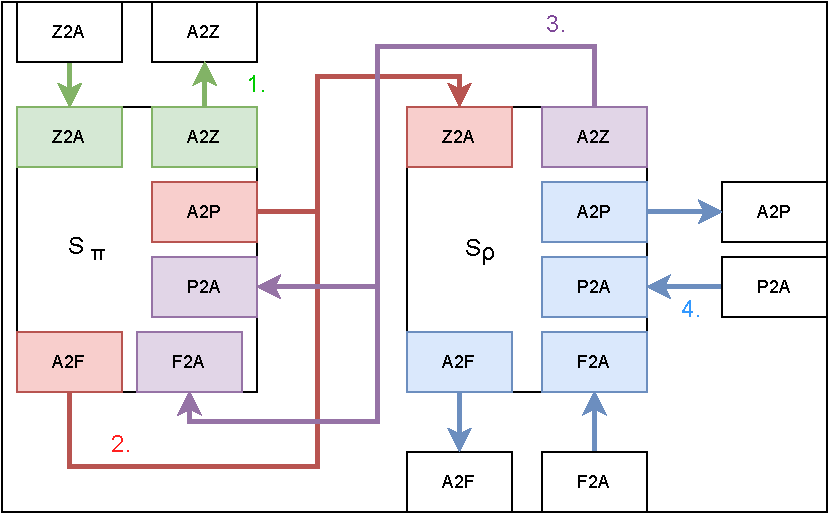
\includegraphics[scale=0.5]{figures/simcomp.pdf}
%\caption{The composed simulators for $\F_1 \xrightarrow{\rho \circ \pi} \F_3$. The real world consists of $(\rho \circ \pi, \F_1)$. Inputs from \Z are for $\F_1$ and dummy parties interacting with $\F_1$, which \SIM{\pi} is equipped to handle. Outputs from \SIM{\pi} are for $\F_2$ and dummy parties of $\F_2$ which \SIM{\rho} is equipped to handle. Finally, outputs from \SIM{\rho} are for $\F_3$ and dummy parties of $\F_3$, which is just the ideal world in Theorem~\ref{thm:composition}.}
%\label{fig:simcomp}
%\end{figure}


\section{Acknowledgment}

%\section*{References}
\bibliographystyle{IEEEtran}
\bibliography{IEEEabrv, saucy}


\newpage

\appendix

\section{Brachs'a Broadcast}
\plan{Commented out: a section describing bracha broadcast}
%\input{sections/bracha}

\section{BenOr's Agreement}
\plan{Commented out: a section describing BenOr}
%\input{sections/benor}

%\section{Software Development in UC}
%In this section we dive into UC as a programming tool for distributed protocols.
We first make the case that the inherent features of UC, namely the real-ideal paradigm and the UC environment and adversarial modelling, are better for specifying, modelling, implementing, and testing distributed systems.
The added benefit of the implementation maintaining a close relationship to a powerful theoretical securuty proof system only bolsters UC's potential as a development environment.
We then go through out process of implementing these protocols in UC and highlight the 


\plan{Add to this first paragraph: in this section we discuss UC and it's tradeoffs/advantages when designing protocols and we leave discussion for testing/verifying implementations for the fuzzing section}
UC is known to be a useful theoretical tool for defining distributed protocols, however crafting definitions in the UC style, whether on-paper or as an implementation, requires careful effort beyond what traditional definitions require.
Like many existing works that have successfully proposed and developed protocols by constraining programmer or protocol behavior~\cite{mace,macemc,farsite,farsiteretro,dbug}, UC imposes a set of rules that change how protocol designers have to think. 
The UC-style mimics maybe of the design principles highlighted by these workd, and, in some respects, takes them further to achieve the similar advantages. 
In this section we relate out experience of translating the ABA Protocol from \cite{ABA} and identify advantages, and some trade-offs, in expressing and implementing protocols in UC.
Namely, we connect the UC framework to existing goals such as modular design, minimization of concurrency hazards, and replayability/determinism of execution.
Furthermore, we note that forcing a programmer or designed to think and frame the problem through this framework forces more careful thought to how protocols may be activated or used incorrectly in a deployment setting---addressing some of the concerns raised by \cite{paxosthoughts} on the usefulness of theoretical model specs and pseudo-code.
Although other frameworks and designs, some of which we reference in this section, achieve similar goals, we argue that UC simulataneously achieves more of them than others, and, the existing gap between theory and practice demands it be taken seriously as a framework worth further exploring.

\textbf{REMEMBER}: An important thing to remember for this section is that we aren't trying to motivate using UC for distributed systems modelling on-paper.
Our point is that designing from a UC-first princiciples:
\begin{itemize} 
\item definitions and code are implemented in a framework that makes it easy to do theoretical work on and proving etc.. when it comes time for it in the future if you're starting with implementation
\item if starting with definitions, UC forces designers to be precise about network assmuptions, models, properties of primitives, adversarial capabilities concretely, how protocol is activated and what happens, initial conditions, etc...
\end{itemize}

% The UC-framework can be described as an event-driven framework with execution without preemption, and a penchant for buggery mr powers\todo{finish}.

% disction between changes required to pseudo code vs changes required in implementation
% in pseudocode you still need to be clear about activations and what to do in certain cases but can be vague about concurrency structure and differen "processes" talking to each other
% in code that has to be made explicit, but pseudocode that outlines how to handle events more specifically means implmenters aren't trying to themselves prove statements to determine what the protocol shoudl o
% for example, a developer aims to make the code as robust as possibleunder arbitrary conditions but the consequences of such choices may be unclear and actually undermine the intent of the paper definition. 
% TODO: the regarding the paxos paper comments on langauge specs or framework for specs are not usually useful in practice --> UC goes some of the way in forcing a designer to think about how to handle realistic scenarios of malformed input or unexpected activation by another process/ITM/message-passing functionality

\subsection{Design Constraints}
Our implementation of the UC framework, doesn't enforce a specific way to write code according to the UC rules and isn't a system that prevents writing ``bad'' code, like \cite{mace} or \cite{verdi}, but it is a set of principles that a programmer must adhere to to reap the benefits that we outline below.
% A similar method is used by Bolosky et al.~\cite{farsite} where the authors iterate through a few design principles and methodolodies to arrive at a way of writing distributed code that maximizes maintanability and modularty and minimizes concurrency hazards and non-determinism.
Of course, our UC implementation places some limitations on what the programmer does: enforcing message types for a protocol/functionality, forcing programmers to use the built-in typeclasses for environments/adversaries/protocols/functionalities, and limiting the ways in which these processes can communicate with each other.
%This approach is similar to the work by Bolosky et al.~\cite{farsite} who work through different iterations of a development framework and set of rules for organizing and writing distributed systems as event handlers. 
%The resulting framework from their efforts, and their ``pinning pattern'', bear a striking resemblance to the the communication rules that UC already implements. 
%Furthermore, their prioritization of preventing concurrency bugs and tackling source of non-determinism are shared by the UC semantics.
%Other works, such as Mace~\cite{mac} and dBug~\cite{dbug}, arrive at similar conclusions and try to instrument distributed code in a modular and layered way so that code is easy to maintain and parts are easy to replace or chop and change. 
%The ideal functionality model, in UC, takes this a step further by not only cleanly abstracting away functionality from lower layers but bridges a gap to theory where many protocols that can realize the same model and interface can be proven, both through theoretical simulation proofs and informal testing of simulators in our implementation, leading to more robust and modular code. 
%A clear example of this advantage arises in \cite{farsite} where nuanced and hard to track bugs arise from their assumptions on quick check implementations accross different operating systens.
%While both were correct, there lacked a clear model and set of properties in mind when implementing their protocol which led to an protocol implementation based on a specific instance of quickcheck rather.
%In the ideal functionality, model, the designer is forced to first undertake choosing an ideal functionality that \emph{succinctly captures the intended properties of a sorting algorith} and assert that the possible candidates that can replace the ideal functionality, when their code is deployed, satisfy some basic simulation properties with the ideal functionalitu or, in the best case, are proven to realize.

%In our experience translating the ABA protocol from ~\cite{aba}, we identify a few key takeaways and trade-offs with expressing protocols in this way. 
%Like existing work~\cite{farsite}, writing code in the UC-style and conforming to its execution rules is not enforced by some type system, but is instead a set of principles that programmers must adhere to.
%Notably, writing paper definitions in the UC styles has the advantage of bringing the paper and its proof closer to the end product: the implmentation.
%Thinking about a protocols as en \emph{event-driven} piece of code force the designed to be explicit about the precise conditions of a protocol party when a new messages is received. 
%Finally, the \emph{write-after-read} semantics of UC ensure that on every event, there is a straight-line and deterministic execution which eliminates a large degree of concurrency hazards that arise in traditional programming. 
%This is a dominant concern, motivation, and goal for existing works that propose frameworks for writing and/or testing code~\cite{farsite, mace, macmc, dbug}, and UC largely addresses most of them already.
%A notable drawback, also pointed out in prior work, is that cosntraints around atomicity of action or a layered approach to programming (like UC's ideal functionality model) stand in the way of high-performance code.
%Though true, we remark that UC is as yet unexplored as a framework for development, and we are only making its case as a candidate for further study in this new domain---challenging the convention wisdom around it.

\paragraph{Modelling Assumptions} 
% POINTS: asynchronous/network assumptions ; assumptions about primitives by using ideal functionalities 
A key advantage of the UC model is that it forces a designer to model both their protocol and the assumed primitives it takes advantage of.
A simple model of the Bracha protocol has to first specify and ideal functionality that exactly captures the intended properties of broadcast.
The model-first approach to system design forces the expected safety, validity, reliability, or timing properties to be clear from the outset.
The Bracha protocol itself exists in a world with a hybrid functionality that described the intended properties expected of the primitives that it uses.
For Bracha broadcast this is a functionality that captures the precise definition of the \emph{asynchronous network} that the protocol assumes it is in.
Not only are timing guaranteed captured, but the ideal functionality defines the adversary's capabilities to delay, reorder, or even modify messages. 

The necessity for designing protocols in a functionality-first way is, first, critical to first ensure systems are not tied to specific implementations~\cite{farsiteretro,farsite} that may change in a different environment (or operating system, for example).
Second, being clear about assumptions, such as precise network modelling, ensures the gap between design/theory and implemenation is minimized. 
In our experience translating the ABA~\cite{ABA} protocol into UC, a big step was ensuring that the minimal asynchronous network asumptions that we implemented the protocol nuder continued to satisfy the intended properties, and there weren't unstated assumptions such as ``all messages in round $r$ are received before round $r+1$''.
Third, we envision a future where there is a large corpus of ideal functionalities and protocols realizing them---proven secure both on paper and in implementations---that programmers can easily plug-in to build larger systems and fall back to UC's compositional security.
% point: you almost end up trying to make the protocol more robust by looking at messages before input is available and you add all these extra steps to the design that are untested or unexplored on paper and you run the risk of departing from the intended behavior. With UC on paper and UC impleenetation and design the gap between the two is much smaller 
\plan{There's something to say about existing works modelling systems in higher-level specs which can be analogous to ideal functionalities}

\todo{talk about some future things in the context of related-works for model specificatios, model checking, etc...}

\paragraph{Realism? (need better heading)}
% POINTS: designs should force encapsulation of spurious events like activation before input ; reduce the gap between specs/definitions/paper and implementation ; less additional work required by programmers ; highlight the benefir in both directions theory <-> implementation
Using UC as a starting and ending point for engineering distributed protocols also overcomes some of frequently mentioned limitations of pseudo-code or on-paper specifications~\cite{paxosthoughts}.
A criticism of such definitions can be that they don't take into account what a program might actuall encounter in the real world.
For example, in the real world programs may be used incorrectly by users or a node's router may temporarily go offline or the program in an agreement protocol might receive messages before it even has a value to propose. 


\plan{Ideal functionalities can't capture any and all properties a designed might want to specify: aba has a property that if all parties have same input then they decide by round r+1. The ideal functionality on its own can't capture timing guarantees like that, so that's a downside but it is still something checkable.}
\todo{Should this point be included in this section, the fuzzing section, or both?}


\paragraph{drafting notes}
There is a statement in the Paxos implementation retrospective that states that often times paper specs aren't very useful for implementation since implementation has to consider so many more things
we state that UC formulation gets you a lot closer by having to be explicit about things like initial conditions, arbitrary message ordering and delivery
UC is useful for theoretical results, but for these reasons that make it good for testing code as well as writing code
it's evidenced by these related works that all attempt to do things very reminiscent of the UC framework but in an ad-hoc way
rather we say that we should consider UC as a candidate for development frameworks rather than them because it achieves largely the same things and supports the same concurrency protection and layering of code and the ideal functionality model provides all these things


\subsection{Implementation Constraints}
Enforcing design and implementation constraints on programmers and designers has tradeoff's as well. 
As referenced by existing work, forcing the programmer into a consrained set of possible designs requires more work and can be cumbersome as well.
Even so, we believe that the advantages of the UC style of programming outweight the disadvanages
Not all the disadvantages are inherent and some may be overcome in future with more focus on this area of research. 



% making explicit the network assumptions in an ideal functionality
%     capturing the properties expected, explicitly
% adding additional handling for initial conditions if activated by fMulticast first
% event-driven programming and read-after-write rules
%     straight-line execution
%     deterministic code path
%     one process activates one-other process
%     "environment activated in betwee" is related to the fuzzing section
  

\section{Fuzz Testing}
\todo{Still need to mention that we use it to test protocol properties and simulator proofs.}
We rely on fuzz testing as our chosen method of informal protocol analysis for a few critical reasons. 
First, there is a wealth of prior work outlinin the success of fuzz testing techniques, even again program verification, for discovering unintended behavior in code.
Second, existing work in fuzz testing often focuses purely on program binaries that do not concurrently communicate with other processes aside from system calls.
A related work to our own, by Jepsen, takes a novel direction by creating a fuzz testing framework for testing the Tendermint byzantine-fault tolerant consensus protocol. 
Here, several nodes communicate with each other through tcp/ip connections and come to consensus on the ordering of messages sent by all the nodes (refer to Section~\ref{sec:relatedworks} for a more in-depth analysis of the work). 
In this work, we attempt a similar mechanism but constrain ourselves to evaluating protocols expressed in the UC framework.
Furthermore, we replicate the work done by jepsen in our framework as a baseline validation for its capabilities. 

\subsection{QuickCheck in with UC}
The QuickCheck module provides primitives for generating input according to some rules. 
The advatage of modelling protocols within the UC framework is that the interface for the adversary's input to the protocol, and any underlying assumptions or network primitives, is made explicit from the start.
This helps constrain the set of possible inputs give to the adversary and make the framework amenable to fuzzing.

\paragraph{Always Enabled Actions}
Part of defining protocols for fuzz testing in \us requires borrowing an idea from Iron Fleet~\cite{ironfleet}.
In standard UC when ITMs normally halt when something goes wrong.
In agreement protocols, a protocol might ensure distinguishability by simply halting when something incorrect happens such as, for example, receiving a broadcast from a part that isn't the sender or running out of import. 
When writing a protocol in \us it is critical that programs don't throw errors or simply stop accepting messages from others, because such situations lead to test runs that hang indefinitely. 
Instead, all prorams need to ensure that all inputs received from other ITMs result in control being passed to another ITM.
In the case of faults, or halting, this simplifies to passing control back to the environment on any input.  \todo{make this better}


\subsection{Creating Test Cases}

\paragraph{Unstructured Environments}
Creating generative environments that follow some type of protocol ordering requires considerable effort and isn't easily done for protocols that take an arbitrary number of rounds.
For example, a structure protocol like the one described for Braca Broadcast necessarily encodes some number of rounds of inputs that are generated. 
A protocol like ABA or the BenOr protocol break this limitation. 
Therefore, we make a more generalized approach to your fuzz testing were we define try to minimize the protocol assumptions made in our generators and determine
whether we can still capture the same bugs in a reasonable amount of time.
Specifically, we examine whether how ``unstructured`` the generator can be and still produce interesting cases (i.e. those where at least some parties decide on a value) and 
how the weight assigned to different inputs in the generator impact this.
We hypothesized that inputs to our asynchronous wrapper (\texttt{ClockA2F_Deliver} and \texttt{ClockA2F_MakeProgress} commands) must be significantly more frequently generates
than honest party input or corrupt party input in order to ensure that the protocol has a high change of making progress.





\subsection{Discovering Safety Bugs in Protocols}
We examine fuzz testing by implementing some classical and a moden byzantine agreement protocol and injecting faults into them.
Most injected bugs arise from misplaces thresholds for parties to take some action.
For example, a protocol that designed to handle $\frac{n}{2}$  

Most injected bugs arise from misplaced thresholds and incorrect assumptions about corrupt party threstholds. 



\subsection{Analyzing Liveness in Distributed Protocols}
Analysis, even informal, about liveness in protocols is a hard problem.
A large body of existing works, like IronFleet, that uses temporal logic to reason 
about some positive actions happening in a distributed protocol, but this comes at 
the cost of significant user.
In this section we explore to what extend our informal analysis of consensus and agreement
protocols, and our implementation of the import mechanism, can discover and give meaningful
feedback about liveness issues to a protocol analyst.

There are some critical limitations in what an informal analysis can achieve.
With the import mechanism, the most interest kinds are evident when the execution runs out
of import, and this leads to a problem of juggling false negatives and false positives when
asking the question: is this protocol live?
Imagine a probabilistic protocol that makes random decisions
and terminates in some expected number of rounds with byzantine agreement. 
For example, say some execution among the generated test cases outputs an error
that some ITM in the execution is out of import. The error can be explained in one of 
two ways:
\begin{enumerate}
	\item The protocol, as defined, does not get enough import from the environment,  or it doesn't pass around enough import between the parties to achieve the desired functionality. It is a randomized protocol and there may be some sequence of random choices that delays termination by a large enough amount (or for many rounds) that the import provided is insufficient. 
	\item The protocol does have a fault, and there is some sequence of random decisions the parties can make which results in the protocol no terminating in a polynomial amount of time. In reality, regardless of the polynomial import provided, there will always be some sequence of decisions that prevents poly-time termination. 
\end{enumerate}
In fact, it may even be the case that in $n$ generate test cases the faulty traces of an incorrect protocol may never be triggered.  

\paragraph{False Negatives}
False negatives occur when a truly live protocol runs out of import trying to terminate. 
In such cases, the natural next analysis step is increasing the polynomial import given
to the protocol until suc 
\todo{hypothesis is that increasing the polynomial and number of test cases reduces false negatives towards zero at the limit}

\paragraph{False Positives}
individual generated executions that report failures may be false negatives for the reasons above.
A fuzz testing run that returns no failure can be false positive as the failure trace hasn't been discovered. 
\todo{hypothesis is that increasing the polynomial and number of test cases approaches a constant upper bound in the limit as the actual traces with never terminate happen infinitely often}



%\pagebreak

\end{document}
